\documentclass[acmsmall,screen]{acmart}

\usepackage{tabularx}
\usepackage{bbm}
\usepackage{mathpartir}
\usepackage{tikz-cd}
\usepackage{xspace}

%\geometry{paperwidth=8.3in, paperheight=11.7in} % force to A4 for now
\settopmatter{printacmref=false}
\citestyle{acmauthoryear}
\raggedbottom

\newcommand*{\note}[1]{\textcolor{blue}{\textbf{note:} #1}}
\newcommand*{\todo}[1]{\textcolor{blue}{\textbf{todo:} #1}}

\newenvironment{salign*}
   {\par\nobreak\small\noindent\csname align*\endcsname}
   {\csname endalign*\endcsname}

\newcommand*{\cat}[1]{\mathbf{#1}}
\newcommand*{\comp}{\circ}
\newcommand*{\eval}{\mathsf{ev}}
\newcommand*{\id}{\mathsf{id}}
\newcommand*{\iso}{\cong}
\newcommand*{\op}{\mathsf{op}}
\newcommand*{\biprod}{\oplus}
\newcommand*{\reindex}[2]{#1[#2]}
\newcommand*{\tensor}{\otimes}
\newcommand*{\zero}{0}

\newcommand*{\One}{\mathbbm{1}}
\newcommand*{\Hom}[3]{{#1}(#2,#3)}

% Specific categories
\newcommand*{\Cat}{\cat{Cat}}
\newcommand*{\CMon}{\cat{CMon}}
\newcommand*{\Fam}{\cat{Fam}}
\newcommand*{\Func}[2]{[#1,#2]}
\newcommand*{\Grothendieck}[1]{\int_{#1}}
\newcommand*{\LatGal}{\cat{LatGal}}
\newcommand*{\Set}{\cat{Set}}
\newcommand*{\Setoid}{\cat{Setoid}}


\begin{document}

\title{Approximation as Differentiation}

\author{Robert Atkey}
\email{robert.atkey@strath.ac.uk}
\orcid{0000-0002-4414-5047}
\affiliation{%
  \institution{University of Strathclyde}
  \city{Glasgow}
  \country{UK}}

\author{Roly Perera}
\email{roly.perera@cl.cam.ac.uk}
\orcid{0000-0001-9249-9862}
\affiliation{%
  \institution{University of Cambridge}
  \city{Cambridge}
  \country{UK}
}
\additionalaffiliation{%
   \institution{University of Bristol}
   \city{Bristol}
   \country{UK}
}

\begin{abstract}
\todo{abstract}
\end{abstract}
\maketitle

\section{Introduction}
\label{sec:introduction}

To audit any computational process, we need robust and well-founded notions of \emph{provenance} to track how data are used. This allows us to answer questions like ``Where did these data come from?'', ``Why are these data in the output?'' and ``How were these data computed?''. Provenance tracking has a wide range of applications, from debugging and program comprehension~\cite{buneman95,cheney07} to improving reproducibility and transparency in scientific workflows~\cite{kontogiannis08}. \emph{Program slicing}, first proposed by~\citet{weiser81}, is a collection of techniques for provenance tracking that attempts to take a run of a program and areas of interest in the output, and turn them into the subset of the input and the program that were responsible for generating those specific outputs.

Existing approaches to program slicing are often tied to particular programming languages or implementations.
In this paper we develop a general categorical approach to program slicing, focusing on a particular technique
called \GPS, where the set of slices of a given value form a lattice of approximations and the forward and
backward slicing procedures generate Galois connections between these lattices. Our main contribution is that
this approach can be seen as a generalised form of automatic differentiation, with slices of values playing
the role of tangents. Our categorical approach should provide a suitable setting for enabling ``automatic''
data provenance for a variety of programming languages, and is easily configured to use alternative
approximation strategies, including quantitative forms of slicing.

\subsection{Galois Program Slicing}
\label{sec:introduction:galois-slicing}

Perera and collaborators introduced the idea of {\em Galois program slicing} as a particular conception of program slicing for provenance, described in several publications~\cite{perera12a,perera16d,ricciotti17}. Galois program slicing (hereafter simply {\emph \GPS}) forms the basis of the open source data visualisation tool \href{https://f.luid.org/}{Fluid}~\cite{perera2025fluid} that allows interactive exploration of programmatically generated visualisations.

At a high level, \GPS assumes that, for each possible value that may be input or output by a program, there exists a lattice of {\em approximations} of that value. For a particular run of a program that takes input $x$ and produces output $y$, we also get a Galois connection between the lattice of approximations of $x$ and the lattice of approximations of $y$. The right half of the Galois connection is the ``forward direction'' taking approximations of the input to approximations of the output; the left half of the Galois connection is the ``backward direction'' that takes approximations of the output to the least (i.e., most approximate) approximation of the input that gives rise to this output approximation. This becomes {\em program slicing} by including the source code of the program as part of the input; then, in the backward direction, the least approximation of the input required for an output approximation includes the least part of the program required as well.

\begin{example}
  \label{ex:introduction-example}
  The following program is written in Haskell syntax \cite{haskell}, using a list comprehension to filter a list of pairs of labels and numbers to those numbers with a given label, and then computing the sum of the numbers:
  \begin{displaymath}
    \begin{array}{l}
      \mathrm{query} :: \mathrm{Label} \to [(\mathrm{Label}, \mathrm{Int})] \to \mathrm{Int} \\
      \mathrm{query}\,l\,\mathit{db} = \mathrm{sum}\,[ n \mid (l',n) \leftarrow \mathit{db}, l \equiv l' ]
    \end{array}
  \end{displaymath}
  With $\mathit{db} = [(\mathsf{a}, 0), (\mathsf{b}, 1), (\mathsf{a}, 1)]$, we will have $\mathit{query}\,\mathsf{a}\,\mathit{db}$ and $\mathit{query}\,\mathsf{b}\,\mathit{db}$ both evaluating to $1$.

  Now suppose that for a given run of the program, we are interested in which of the numerical parts of the input are used to compute the output for the query parameters $l = \mathsf{a}$ and $l = \mathsf{b}$. We can use \GPS to do this. We arrange for the approximations of the input to form the following lattice, where the actual piece of data is at the top and information lost by approximation is represented by $\bot$s:
  \begin{center}
    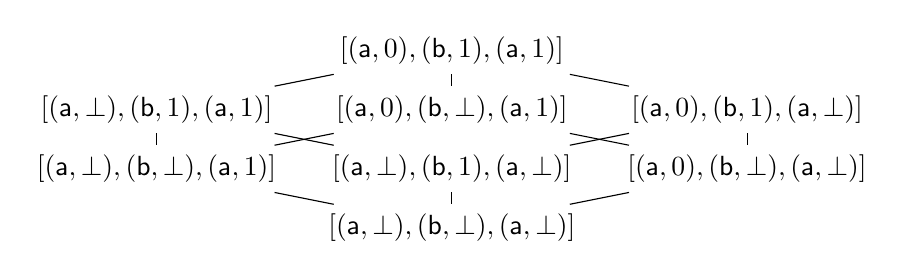
\begin{tikzpicture}[node distance=0.75cm]
      \node (top) at (0,0) {$[(\mathsf{a}, 0), (\mathsf{b}, 1), (\mathsf{a}, 1)]$};
      % row 2
      \node [below of=top] (ioi) {$[(\mathsf{a}, 0), (\mathsf{b}, \bot), (\mathsf{a}, 1)]$};
      \node [left of=ioi,xshift=-3cm] (oii) {$[(\mathsf{a}, \bot), (\mathsf{b}, 1), (\mathsf{a}, 1)]$};
      \node [right of=ioi,xshift=3cm] (iio) {$[(\mathsf{a}, 0), (\mathsf{b}, 1), (\mathsf{a}, \bot)]$};
      % row 3
      \node [below of=ioi] (oio) {$[(\mathsf{a}, \bot), (\mathsf{b}, 1), (\mathsf{a}, \bot)]$};
      \node [left of=oio,xshift=-3cm] (ooi) {$[(\mathsf{a}, \bot), (\mathsf{b}, \bot), (\mathsf{a}, 1)]$};
      \node [right of=oio,xshift=3cm] (ioo) {$[(\mathsf{a}, 0), (\mathsf{b}, \bot), (\mathsf{a}, \bot)]$};
      % row 4
      \node [below of=oio] (bot) {$[(\mathsf{a}, \bot), (\mathsf{b}, \bot), (\mathsf{a}, \bot)]$};

      % links
      \draw (top) -- (ioi);
      \draw (top) -- (oii);
      \draw (top) -- (iio);
      \draw (ioi) -- (ooi);
      \draw (ioi) -- (ioo);
      \draw (oii) -- (ooi);
      \draw (oii) -- (oio);
      \draw (iio) -- (ioo);
      \draw (iio) -- (oio);
      \draw (ooi) -- (bot);
      \draw (oio) -- (bot);
      \draw (ioo) -- (bot);
    \end{tikzpicture}
  \end{center}
  In both runs of the program, the output approximation lattice looks like this, where $1$ is the actual data point that was returned, and $\bot$ indicates that we are approximating this piece of data away:
  \begin{center}
    \begin{tikzpicture}[node distance=0.75cm]
      \node (top) at (0,0) {$1$};
      \node [below of=top] (bot) {$\bot$};
      \draw (top) -- (bot);
    \end{tikzpicture}
  \end{center}
  These are not the only choices of approximation lattices that we could have made. For the input, we have chosen a lattice that allows us to ``forget'' (approximate away) numbers in the input, but not the labels or the structure of the list itself. However, other choices are also useful. Indeed, one of the aims of this work is to clarify how to choose an approximation structure appropriate for different tasks by use of type information. We elaborate on this further in \secref{semantic-gps}.

  \GPS associates with each run of the program a Galois connection telling us how the inputs and outputs are related in that run. The backwards portion $\partial (\mathit{query}\,l)_r$ tells us, given an approximation of the output, what the least approximation of the input is needed to generate that output. In the case of the two runs considered in this example, if we say we are not interested in the output by feeding in the least approximation $\bot$, then we find that we only need the least approximation of the input:
  \begin{displaymath}
    \partial (\mathit{query}\,l\,\mathit{db})_r(\bot) = [(\mathsf{a},\bot), (\mathsf{b}, \bot), (\mathsf{a}, \bot)]
  \end{displaymath}
  for both $l = \mathsf{a}$ and $l = \mathsf{b}$. If instead we take the greatest approximation of the output (i.e., the output ``$1$'' itself), then the two query runs' backwards approximations return different results:
  \begin{displaymath}
    \begin{array}{l}
      \partial (\mathit{query}\,\mathsf{a}\,\mathit{db})_r(1) = [(\mathsf{a},0), (\mathsf{b},\bot), (\mathsf{a},1)] \\
      \partial (\mathit{query}\,\mathsf{b}\,\mathit{db})_r(1) = [(\mathsf{a},\bot), (\mathsf{b},1), (\mathsf{a},\bot)]
    \end{array}
  \end{displaymath}
  Pieces of the input that were {\em not} used are replaced by $\bot$. As we expect, the run of the query with label $\mathsf{a}$ depends on the entries in the database labelled with $\mathsf{a}$, and likewise for the run with label $\mathsf{b}$.

  In this case, the forwards portion of the Galois connection tells us, for each approximation of the input, whether or not it is sufficient to compute the output. If we provide insufficient data to compute the output, then we will get an underapproximated output. Here for example we will find that $\partial (\mathit{query}\, \mathsf{a})_f([(\mathsf{a},0),(\mathsf{b},\bot),(\mathsf{a},\bot)]) = \bot$ because we need all the values associated with the label $\mathsf{a}$ to compute their sum.

  In a simple query like this, it is easy to work out the dependency relationship between the input and output. However, the benefit of \GPS, and other language-based approaches, is that it is {\em automatic} for all programs, no matter how complex the relationship between input and output. Moreover, by changing what we mean by ``approximation'' we can compute a range of different information about a program.
\end{example}

\subsection{Galois Slicing and Automatic Differentiation}

Previous work on \GPS used a special operational semantics to generate a trace of each execution, and then uses that trace to compute the Galois connections described above, by re-running forwards or backwards over the trace. It would be useful to have a denotational account of \GPS as well, especially if we could provide a semantics where the backwards analysis is baked in, rather than provided by a separately defined ``backwards evaluation'' operation. Our thesis, developed in \secref{approx-as-tangents} and \secref{models-of-total-gps} is that there is a close analogy between \GPS and \emph{automatic differentiation} for differentiable programs~\cite{siskind08,elliott18,vakar22}, which points to a way to develop such an approach. We have already hinted at this in the description above, but let us now make it explicit.

\begin{itemize}[leftmargin=\enummargin]
\item For \GPS, we assume that every value has an associated lattice of {\em approximations}. For differentiable programs, every point has an associated vector space of {\em tangents}.
\item For \GPS, every program has an associated forward approximation map that takes approximations forward from the input to the output. This map {\em preserves meets}. For differentiable programs, every program has a forward derivative that takes tangents of the input to tangents of the output. The forward derivative map is {\em linear}, so it preserves addition of tangents and the zero tangent.
\item For \GPS, every program has an associated backward approximation map that takes approximations of the output back to least approximations of the input. This map {\em preserves joins}. For differentiable programs, every program has a reverse derivative that takes tangents of the output to tangents of the input. This map is again {\em linear}.
\item For \GPS, the forward and backward approximation maps are related by being a Galois connection. For differentiable programming, the forward and reverse derivatives are related by being each others' transpose.
\end{itemize}

Given this close connection between \GPS and differentiable programming, we can take structures intended for modelling automatic differentiation, such as V{\'a}k{\'a}r's CHAD framework and use them to model \GPS. This will enable us to generalise and expand the scope of \GPS to act as a foundation for data provenance in a wider range of computational settings.

\subsection{Outline and Contributions}

%Our primary contribution in this article is to elucidate \GPS by relating it to differentiable programming and automatic differentiation. In doing so, we aim to expand the applicability of program slicing, and to potentially transfer efficient automatic differentiation implementation techniques from automatic differentiation to program slicing and provenance tracking.

\GPS, as any program slicing technique, essentially rests on an analysis of how programs intensionally explore their input, in addition to their extensional behaviour. Such analysis has been carried out over many years in Domain Theory. In \secref{approx-as-tangents}, we use ideas from \citet{berry79}'s \emph{stable domain theory} and develop an analogy between stable functions and smooth functions from mathematical analysis, where stable functions provide a kind of semantic provenance analysis. In \secref{models-of-total-gps}, we abstract from stable functions using V{\'a}k{\'a}r \etal{}'s CHAD framework \cite{vakar22,nunes2023} to build models of a higher-order language that automatically compute slices. We apply this to a concrete higher-order language in \secref{language} and demonstrate the use of the model on variations of \exref{introduction-example}, highlighting the flexibility of our approach. In particular, we show how type structure can be used to control the approximation lattices associated with data points, something that was ``hard coded'' in previous presentations of \GPS. We prove two correctness properties in \secref{definability}, relating the higher-order interpretations to first-order ones, proving the crucial Galois connection property. \secref{related-work} and \secref{conclusion} discuss additional related and future work.

% \begin{enumerate}[leftmargin=\enummargin]
% \item We explain how the CHAD framework of Vákár et al. can be adapted to give a general categorical framework for \GPS.
% \item Using our adapted CHAD framework, we can explain how type structure can be used to control the approximation lattices associated with data points, something that was ``hard coded'' in previous presentations of \GPS.
% \item With the benefit of our abstract setting, we can relate \GPS to other parts of denotational semantics. In particular, we show that there is a close connection with Stable Domain Theory, a proposed solution to capturing sequentiality by recording more intensional information about programs' sensitivity to approximations.
% \end{enumerate}

We have formalised our major results in Agda, resulting in an executable implementation built directly from the categorical constructions that we have used to compute the examples in \secref{language:examples}. Please consult the file \texttt{everything.agda} in the supplementary material.


% \begin{enumerate}
% \item We explain how the CHAD framework of Vákár et al. can be adapted to give a general categorical framework for \GPS.
% \item Using our adapted CHAD framework, we can explain how type structure can be used to control the approximation lattices associated with data points, something that was ``hard coded'' in previous presentations of \GPS.
% \item With the benefit of our abstract setting, we can relate \GPS to other parts of denotational semantics. In particular, we show that there is a close connection with Stable Domain Theory, a proposed solution to capturing sequentiality by recording more intensional information about programs' sensitivity to approximations.

% We have \anonymise{\href{https://github.com/bobatkey/approx-diff}{formalised this work in Agda}}{formalised this work in Agda}. Not only does this mean that the constructions and proofs have been checked, but also the construction is executable and can be run on small examples. We are also planning to use Agda's JavaScript backend to produce a demo.

\section{Formal Structures for Generalised Automatic Differentiation}

\note{Probably a better way: (1) introduce the category of lattices and Galois connections, which is what we will use to interpret forward and backward approximation, and establish some properties of this category; (2) say that we want sets with each point having an associated lattice of approximations, and morphisms to match; (3) note that this is exactly the Grothendieck construction for a particular indexed category; (4) Say that CHAD is what we need here; (5) Recapitulate the bits of CHAD that we need, with our Agda formalisation; (6) Explain how we cope with higher-order structure, by using presheaves and the Yoneda embedding.}

We take an approach based on the CHAD (Combinatory Homomorphic Automatic Differentiation) of Mattias Vákár and others \cite{nunes2023}. Here follows a rough overview of this approach and how we have applied it to Galois program slicing. \todo{Final version shouldn't be ``rough''!}

We have \href{https://github.com/bobatkey/approx-diff}{formalised this work in Agda}. Not only does this mean that the constructions and proofs have been checked, the construction is executable and can be run on small examples. We are also planning to use Agda's JavaScript backend to produce a demo.\todo{Do this?}

The fundamental approach in CHAD is to consider Grothendieck constructions on indexed categories $T : \cat{C}^\op \to \Cat$. An object of the Grothendieck construction $\int T$~, described in more detail in \secref{Grothendieck}, is a pair $(X \in \cat{C}, \partial X \in T(X))$, which we read as pairing a space $X$ of ``points'' from $\cat{C}$ with an associated bundle of tangent spaces. The maps from the ``base'' category $\cat{C}$ are used to interpret the programs we are modelling. The maps in the indexed category are the maps of tangents or approximations, being derivatives and Galois connections respectively.

In the case of differentiable programs and automatic differentiation, a basic model can be constructed by taking $\cat{C}$ to be $\Set$ and $T(X) = X \to \FinVect$: indexed collections of finite dimensional vector spaces, whose elements are interpreted as tangents at the given point, with linear maps. The Grothendieck category $\int T$ has objects that are pairs of a set $X$ and for each $x \in X$ a tangent vector space $\partial X(x)$. Morphisms are pairs of maps of points to points, accompanied by linear maps of tangents at those points. If we carefully choose an initial set of maps, we can read these maps as derivatives (note that nothing in the Grothendieck construction says that they must be derivatives!). Composition in the Grothendieck category is exactly the {\em chain rule} for composing derivatives, so we at least do know that if we start with derivatives on basic operations, then composing them will retain this property.

For Galois program slicing, we again take $\cat{C}$ to be $\Set$ and now take $T(X) = X \to \LatGal$: indexed collections of lattices, whose elements are interpreted as approximations at the given point, with indexed Galois connections as the maps between them.

In these special cases when $\cat{C} = \Set$, the Grothendieck construction is the {\em families} constructions $\Fam(\FinVect)$ and $\Fam(\LatGal)$~(\secref{Fam}). As is well known~\cite{lawvere63}, $\Fam(\cat{X})$ for any category $\cat{X}$ is the free coproduct completion of $\cat{X}$. In the case that $\cat{X}$ has a (symmetric) monoidal product, then we always get a symmetric monoidal product on $\Fam(\cat{X})$ (using the Cartesian products from $\Set$). When $\cat{X}$ has all (small) products, and the monoidal product is actually a coproduct, then $\Fam(\cat{X})$ is symmetric monoidal closed. If the coproducts are actually {\em biproducts}~(\secref{biproducts}), then $\Fam(\cat{X})$ is Cartesian closed, and we can interpret higher-order programs.

Happily, $\FinVect$ and $\LatGal$ both have biproducts, as a consequence of them having products and being enriched in commutative monoids\todo{fwd ref}. However, neither of them has all small products, without moving to infinite dimensional vector spaces (in the case of $\FinVect$) or complete lattices (in the case of $\LatGal$). Neither of these are ideal. In infinite dimensional vector spaces, dualisation is not involutive and the connection between the forward and reverse derivatives is lost. In complete lattices, we can no longer easily implement the infinite meets and joins required, and we lose the computability of the model. Moreover, in Agda, there are issues with predicativity when considering complete lattices.\todo{be more specific}

Vákár overcomes this by using different interpretations for forward and backward derivatives. we overcome this by using $\CMon$-enriched presheaves.\todo{elaborate.}

\subsection{Category of lattices and Galois connections}

First we introduce the category of lattices and Galois connections, which will serve as our base category for
interpreting forward and backward Galois slicing. Galois connections are pairs of monotone functions $f: Y \to
X$ and $g: X \to Y$ between posets, where $f$ is the (pointwise) best approximation from below to an inverse
of $g$, and $g$ the best approximation from above to an inverse of $f$. This setup is a nice fit for the
bidirectional nature of (dynamic) program slicing, with $f$ capturing \emph{backward} slicing (producing the
least input slice for a given slice of the output), and $g$ capturing \emph{forward} slicing (producing the
greatest output slice for a given slice of the input).

\begin{definition}[Galois connection]
Suppose $X$ and $Y$ are posets. A \emph{Galois connection} $f \adj g: X \to Y$ is a pair of monotone functions
$f: Y \to X$ and $g: X \to Y$ satisfying $y \leq g(x) \iff f(y) \leq x$ for any $x \in X$ and $y \in Y$.
\end{definition}

\noindent Galois connections thus generalise order isomorphisms. The $\adj$ notation is justified because a
Galois connection $f \adj g: X \to Y$ can also be seen an adjunction between poset categories, with monotone
$f$ and $g$ interpreted as functors; $f$ is usually referred to as the \emph{upper} (right) adjoint and $g$ as
the \emph{lower} (left) adjoint. Galois connections compose component-wise, with $\id_X \adj \id_X: X \to X$
as the unit for composition, and thus form a category $\PosGal$ with all posets as objects and all Galois
connections between them as morphisms.

As sketched in \secref{introduction:galois-slicing}, for Galois slicing we want a setting where the
approximants of a point $x$ form a bounded lattice $(X, \meet, \join, \top, \bot)$, with least element $\bot$
representing the approximation that discards all information about $x$, greatest element $\top$ representing
the approximation that retains all information about $x$, and $\meet$ and $\join$ providing two canonical ways
to combine approximations. Thus rather than working directly in $\PosGal$, we consider the following
subcategory instead.

\begin{definition}
Define $\LatGal$ to be the category which has as objects $X = (X, \meet, \join, \top, \bot)$ all bounded
lattices, and as morphisms all Galois connections $f \adj g: X \to Y$.
\end{definition}

\noindent Right adjoints preserves limits and left adjoints preserves colimits, so for any $f \adj g: X \to Y$
in $\LatGal$, $g$ is a (bounded) \emph{meet-semilattice homomorphism}, i.e.~preserves the meet-semilattice
structure $(X, \meet, \top)$. Similarly, $f$ is a join-semilattice homomorphism with respect to $(X, \join,
\bot)$.

The meet-semilattice homomorphisms from $X$ to $Y$ form a meet-semilattice themselves, with $\meet$ on
homomorphisms defined pointwise, so that $(f \meet g)(x) = f(x) \meet g(x): X \to Y$, and the constant map
$\top_{X,Y}: X \to Y$ sending any $x \in X$ to $\top_Y$ providing the unit (and both preserving meets). Dually
the join-preserving maps from $Y$ to $X$ have a join-semilattice structure given pointwise by $\join$ and the
constant homomorphism $\bot_{Y,X}: Y \to X$ sending any $y \in Y$ to $\bot_X$. Since these two constructions
come in adjoint pairs, $\LatGal$ is enriched in the category $\SemiLat$ of semilattices and semilattice
homomorphisms. The hom-set $\LatGal(X,Y)$ forms a bounded meet semilattice with unit $\top_{X,Y}$ given by the
Galois connection $\bot_{Y,X} \adj \top_{X,Y}: X \to Y$ and meet of Galois connections $(f \adj g) \meet (f'
\adj g') = (f \join f') \adj (g \meet g'): X \to Y$.

Another notable property of $\LatGal$ is that the projections $\pi_1: X \times Y \to X$ and $\pi_2: X \times Y
\to Y$, where $X \times Y$ denotes the product of lattices, have both upper and lower adjoints. This means $X
\times Y$, which we shall hereafter write as $X \biprod Y$, acts as both a product and a coproduct, with
projections $\biproj_X$ and $\biproj_Y$ and injections $\biinj_X$ and $\biinj_Y$ given by:

\vspace{-4mm}
\begin{minipage}[t]{0.45\textwidth}
\begin{center}
\begin{align*}
   \biproj_X = \prodM{\id_X}{\bot_Y} \adj \proj_1: X \biprod Y \to X \\
   \biproj_Y = \prodM{\bot_X}{\id_Y} \adj \proj_2: X \biprod Y \to Y
\end{align*}
\end{center}
\end{minipage}%
\begin{minipage}[t]{0.45\textwidth}
\begin{center}
\begin{align*}
   \biinj_X = \pi_1 \adj \prodM{\id_X}{\top_Y} : X \to X \biprod Y \\
   \biinj_Y = \pi_2 \adj \prodM{\top_X}{\id_Y}: Y \to X \biprod Y
\end{align*}
\end{center}
\end{minipage}
\vspace{2mm}

\noindent The trivial 1-point lattice, which is both terminal and initial, is the unit for $\biprod$. Although
the presence of biproducts is incompatible with $\LatGal$ itself being Cartesian closed, the biproduct
structure will prove crucial for establishing a Cartesian closed setting for interpreting higher-order
programs for Galois slicing.

\subsection{A categorical framework for Galois slicing}

We will consider a pure, total language, where types can be interpreted as sets. Our goal is to equip the
interpretations of programs with Galois connections relating approximations of their inputs to approximations
of their outputs. Since these lattices of approximations depends on the value being approximated, the
semantics of every type $\tau$ must have both a ``conventional'' component, providing the set $X$ associated
with $\tau$, plus an associated lattice of approximations $\partial X(x)$ for every point $x \in X$. The
semantics of an expression $e$ of type $Y$ with a single free variable of type $X$ must then also have two
components: a function $f: X \to Y$ giving the baseline (unapproximated) meaning of the expression, plus a
family of Galois connections $\partial f(x): \partial X(x) \to \partial Y(f(x))$ for every $x \in X$ which can
be used for slicing over that expression.

\subsubsection{Grothendieck construction for indexed categories}
\label{sec:Grothendieck}

This pattern of objects and morphisms is exactly the \emph{Grothendieck construction} for a particular indexed
category $T: \Set^\op \to \Cat$, namely the functor which assigns to every set $X$ the functor category $T(X)
= \Func{X}{\LatGal}$. Here the (discrete) category $X$ is a plain set and so $\Func{X}{\LatGal}$ is exactly
the category of $X$-indexed families of bounded lattices, with $X$-indexed families of Galois connections
between them as morphisms. The Grothendieck construction $\Grothendieck{}T$~(\defref{Grothendieck} below) is
the category of all $\Set$-indexed families of bounded lattices, together with morphisms that account for both
structure within each family and how families transform under reindexing.

First we formalise $X$-indexed families and their categories.

\begin{definition}[Category of $X$-indexed families]
For any set $X$ (interpreted as a discrete category) and any category $\cat{C}$, recall that the functor
category $\Func{X}{\cat{C}}$ has as objects all functors $F: X \to \cat{C}$, namely $X$-indexed families of
objects of $\cat{C}$, and as morphisms from $F \to G$, all families of morphisms $\eta(x): F(x) \to G(x)$ in
$\cat{C}$ for every $x \in X$, with naturality trivial because $X$ only has identity morphisms.
\end{definition}

Like any functor category $\Func{X}{\cat{C}}$ inherits limits and colimits from its codomain.

\begin{proposition}
If $\cat{C}$ has limits (resp.~colimits) then $\Func{X}{\cat{C}}$ has limits (resp.~colimits) computed
pointwise.
\end{proposition}

\begin{definition}[Reindexing]
For any function $f: X \to Y$ define the \emph{reindexing} functor $\reindex{-}{f}: \Func{Y}{\cat{C}} \to
\Func{X}{\cat{C}}$ which sends any $Y$-indexed family $F$ over $\cat{C}$ to the $X$-indexed family
$\reindex{F}{f} = F \comp f$ (regarding $f$ as a functor between $X$ and $Y$ as discrete categories) and any
family of morphisms $\eta: F \to G$ to $\reindex{\eta}{f}: \reindex{F}{f} \to \reindex{G}{f}$ with
$\reindex{\eta}{f}(x) = \eta(f(x))$.
\end{definition}

Although reindexing is just precomposition with $f$, writing it as $\reindex{-}{f}$ avoids notational
confusion when combining composition of morphisms in $\Func{X}{C}$ with reindexing.

\begin{definition}
\label{def:Grothendieck}
Suppose an indexed category $T: \cat{C}^\op \to \Cat$. The \emph{Grothendieck construction} for $T$ is the
category $\Grothendieck{X}T(X)$ (also written $\Grothendieck{}T$) which has as objects, all pairs $(X,
\partial X)$ of an object $X$ of $\cat{C}$ and an object $\partial X$ of $T(X)$, and as morphisms $(X,
\partial X) \to (Y, \partial Y)$, all pairs $(f, \partial f)$ of morphisms $f: X \to Y$ in $\cat{C}$ and
morphisms $\partial f: \partial X \to T(f)(\partial Y)$ in $T(X)$.
\end{definition}

\noindent The $\partial X$ notation is intended to suggest the connection between the Grothendieck
construction and the idea of tangent spaces and derivatives. To understand how the $\partial f$ components
compose, consider any $(f, \partial f): (X, \partial X) \to (Y, \partial Y)$ and $(g, \partial g): (Y,
\partial Y) \to (Z, \partial Z)$ in $\Grothendieck{}T$. We have:

\begin{itemize}
\item $\partial f: \partial X \to T(f)(\partial Y)$, and
\item $T(f)(\partial g): T(f)(\partial Y) \to T(f)(T(g)(\partial Z)) = T(g \comp f)(\partial Z)$
\end{itemize}

\noindent where $T(f)(\partial g)$ is the image of $\partial g$ in the ``reindexing'' functor $T(f)$. The
composition $(g, \partial g) \comp (f, \partial f): (X, \partial X) \to (Z, \partial Z)$ is then given by $(g
\comp f, T(f)(\partial g) \comp \partial f)$.

\subsubsection{Category of families}
\label{sec:Fam}

Of interest to us is the Grothendieck construction for $\Func{-}{\cat{C}}: \Set^{\op} \to \Cat$, the indexed
category which sends any set $X$ to the category of $X$-indexed families $\Func{X}{\cat{C}}$ and any function
$f: X \to Y$ to the reindexing functor $\reindex{-}{f}: \Func{Y}{\cat{C}} \to \Func{X}{\cat{C}}$ .

\begin{definition}[Category of families]
\label{def:Fam}
For any category $\cat{C}$ define $\Fam(\cat{C})$ to be the Grothendieck construction
$\Grothendieck{X}\Func{X}{\cat{C}}$.
\end{definition}

\noindent In $\Fam(\cat{C})$ the objects $(X, \partial X)$ are thus sets $X$ paired with indexed families
$\partial X: X \to \cat{C}$ and morphisms $(f, \partial f): (X, \partial X) \to (Y, \partial Y)$ are functions
$f: X \to Y$ paired with morphisms $\partial f: \partial X \to \partial \reindex{Y}{f}$ in
$\Func{X}{\cat{C}}$.

\subsubsection{Galois slicing via the Grothendieck construction}

Now consider the total category $\Fam(\LatGal)$, which is our basic setting for interpreting first-order
programs for Galois slicing. This has as objects $(X, \partial X)$, all pairs of a set $X$ and and for every
$x \in X$, a bounded lattice $\partial X(x)$, and as morphisms $(X, \partial X) \to (Y, \partial Y)$, all
pairs $(f, \partial f)$ of a function $f: X \to Y$ and for every $x \in X$, a Galois connection $\partial
f(x): \partial X(x) \to \partial Y(f(x))$, as required. The pullback (reindexing) along $f$ in the composition
$(g, \partial g) \comp (f, \partial f) = (g \comp f, \reindex{\partial g}{f} \comp \partial f)$ selects the
appropriate lattice of approximations and Galois connection at each point, using the baseline (unapproximated)
function $f$.

\subsection{Biproducts and Semi-Additive Categories}
\label{sec:biproducts}

We noted that $\LatGal$ is enriched in $\CMon$, the category of commutative monoids (in fact in $\SemiLat$)
and moreover that the product of lattices is also a coproduct, making $\LatGal$ into a category with
\emph{biproducts}. In fact the presence of biproducts is sufficient for $\CMon$-enrichment; such a category is
called \emph{semi-additive}.

\begin{definition}[Semi-additive category]
A category with finite products and coproducts is \emph{semi-additive} if the canonical morphisms (projections
and injections) give an isomorphism
\[\textstyle X \coprod Y \iso X \prod Y\] that is natural in both variables.
\end{definition}

The product/coproduct is called a \emph{biproduct}, with the biproduct structure denoted by $(\biprod, 0)$.
The unit $0$ is both terminal and initial and is called a \emph{zero} object. \todo{State the biproduct
``laws'' that follow from this formulation.} A semi-additive category $\cat{C}$ is enriched in $\CMon$: for
any two morphisms $f, g: X \to Y$ in $\cat{C}$, the biproduct structure provides a way to ``add'' them
together, forming a morphism $f + g: X \to Y$. Diagrammatically:

\begin{center}
\begin{tikzcd}
   X \arrow[r, "\diag"] & X \biprod X \arrow[r, "f \biprod g"] & Y \biprod Y \arrow[r, "\codiag"] & Y
\end{tikzcd}
\end{center}

Here $\diag$ denotes the diagonal $\prodM{\id_X}{\id_X}$ given by the universal property of the product and
$\codiag$ denotes the codiagonal $\coprodM{\id_X}{\id_Y}$ given by the universal property of the coproduct.
The $f \oplus g$ morphism is the component-wise map $\prodM{f \comp \pi_1}{g \comp \pi_2} = \coprodM{\inj_1
\comp f}{\inj_2 \comp g}$. Similarly we can exhibit a \emph{zero} morphism $0_{X,Y}$ by composing the unique
maps in and out of the zero object:

\begin{center}
\begin{tikzcd}
   X \arrow[r, "!_X"] & 0 \arrow[r, "!^Y"] & Y
\end{tikzcd}
\end{center}

It is easy to verify that $+$ is associative and commutative and that $f + 0_{X,Y} = f$, and thus that every
hom-object $\cat{C}(X,Y)$ is an object in $\CMon$. Moreover composition is \emph{bilinear}, i.e.~given by a
family of morphisms $\Hom{\cat{C}}{Y}{Z} \tensor \Hom{\cat{C}}{X}{Y} \to \Hom{\cat{C}}{X}{Z}$ in $\CMon$ that
preserve the additive structure in $\Hom{\cat{C}}{Y}{Z}$ and $\Hom{\cat{C}}{X}{Y}$ separately:

\begin{salign*}
f \comp \zero_{X,Y} = 0_{X,Z} = \zero_{Y,Z} \comp f
\end{salign*}
\begin{salign*}
(f + g) \comp h &= (f \comp h) + (g \comp h) \\
h \comp (f + g) &= (h \comp f) + (h \comp g)
\end{salign*}

\subsection{Grothendieck Construction for Indexed Categories}
\label{sec:Grothendieck}

The goal now is to equip the interpretation of a (first-order) program with a Galois connection relating
approximations of its inputs to approximations of its output. Since the specific lattices of approximations
depend on the value being approximated, the semantics of every type $\tau$ must have both a conventional
component as well as an approximating component, i.e.~a set $X$ which serves as the usual interpretation of
$\tau$, plus an associated lattice of approximations $\partial X(x)$ for every point $x \in X$. The semantics
of an expression $e$ of type $\sigma$ with a single free variable of type $\tau$ (with $\tau$ and $\sigma$
denoting $X$ and $Y$) must then also have two components: a function $f: X \to Y$ giving the conventional
interpretation of $e$, plus a family of Galois connections $\partial f(x): \partial X(x) \to \partial Y(f(x))$
for every $x \in X$ which can be used for slicing over that expression.

This pattern of objects and morphisms is captured by the construction used in CHAD~\cite{vákár22,nunes2023} to
model automatic differentiation, namely the \emph{Grothendieck construction} for a particular set-indexed
category $T: \Set^\op \to \Cat$. For automatic differentiation, $T(X)$ will be the functor category
$\Func{X}{\FinVect}$, regarded as the category of $X$-indexed families of finite vector spaces, with indexed
linear maps as morphisms. For Galois slicing, we will take $T(X) = \Func{X}{\LatGal}$, the category of
$X$-indexed families of bounded lattices, with indexed Galois connections as morphisms.

The Grothendieck construction $\Grothendieck{}T$~(\defref{Grothendieck} below) for an indexed category $T$,
sometimes called the \emph{total category} for $T$, is the category of all set-indexed families of objects of
$T$, together with morphisms that account for both structure within each family and how families transform
under reindexing functions $f: X \to Y$. First we formalise $X$-indexed families and their categories.

\begin{definition}[Category of $X$-indexed families]
For any set $X$ (regarded as a discrete category) and any category $\cat{C}$, recall that the functor
category $\Func{X}{\cat{C}}$ has as objects all functors $F: X \to \cat{C}$, namely $X$-indexed families of
objects of $\cat{C}$, and as morphisms from $F \to G$, all families of morphisms $\eta(x): F(x) \to G(x)$ in
$\cat{C}$ for every $x \in X$, with naturality trivial because $X$ has only identity morphisms.
\end{definition}

Like any functor category $\Func{X}{\cat{C}}$ inherits limits and colimits pointwise from its codomain.

\begin{proposition}
If $\cat{C}$ has limits (resp.~colimits) then $\Func{X}{\cat{C}}$ has limits (resp.~colimits) computed
pointwise.
\end{proposition}

\begin{definition}[Reindexing]
For any function $f: X \to Y$ define the \emph{reindexing} functor $\reindex{-}{f}: \Func{Y}{\cat{C}} \to
\Func{X}{\cat{C}}$ which sends any $Y$-indexed family $F$ over $\cat{C}$ to the $X$-indexed family
$\reindex{F}{f} = F \comp f$ (regarding $f$ as a functor between $X$ and $Y$ as discrete categories) and any
family of morphisms $\eta: F \to G$ to $\reindex{\eta}{f}: \reindex{F}{f} \to \reindex{G}{f}$ with
$\reindex{\eta}{f}(x) = \eta(f(x))$.
\end{definition}

Although reindexing is just precomposition with $f$, writing it as $\reindex{-}{f}$ avoids notational
confusion when combining composition of morphisms in $\Func{X}{C}$ with reindexing.

\begin{definition}
\label{def:Grothendieck}
\todo{Move earlier because doesn't assume $\cat{C} = \Set$.} Suppose an indexed category $T: \cat{C}^\op \to
\Cat$. The \emph{Grothendieck construction} for $T$ is the category $\Grothendieck{X}T(X)$ (also written
$\Grothendieck{}T$) which has as objects, all pairs $(X, \partial X)$ of an object $X$ of $\cat{C}$ and an
object $\partial X$ of $T(X)$, and as morphisms $(X, \partial X) \to (Y, \partial Y)$, all pairs $(f, \partial
f)$ of morphisms $f: X \to Y$ in $\cat{C}$ and morphisms $\partial f: \partial X \to T(f)(\partial Y)$ in
$T(X)$.
\end{definition}

\noindent The $\partial X$ notation is intended to suggest the connection between the Grothendieck
construction and the idea of tangent spaces and derivatives. To understand how the $\partial f$ components
compose, consider any $(f, \partial f): (X, \partial X) \to (Y, \partial Y)$ and $(g, \partial g): (Y,
\partial Y) \to (Z, \partial Z)$ in $\Grothendieck{}T$. We have:

\begin{itemize}
\item $\partial f: \partial X \to T(f)(\partial Y)$, and
\item $T(f)(\partial g): T(f)(\partial Y) \to T(f)(T(g)(\partial Z)) = T(g \comp f)(\partial Z)$
\end{itemize}

\noindent where $T(f)(\partial g)$ is the image of $\partial g$ in the ``reindexing'' functor $T(f)$. The
composition $(g, \partial g) \comp (f, \partial f): (X, \partial X) \to (Z, \partial Z)$ is then given by $(g
\comp f, T(f)(\partial g) \comp \partial f)$.

\subsection{Category of Families}
\label{sec:Fam}

Of interest to us is the Grothendieck construction for $\Func{-}{\cat{C}}: \Set^{\op} \to \Cat$, the indexed
category which sends any set $X$ to the category of $X$-indexed families $\Func{X}{\cat{C}}$ and any function
$f: X \to Y$ to the reindexing functor $\reindex{-}{f}: \Func{Y}{\cat{C}} \to \Func{X}{\cat{C}}$ .

\begin{definition}[Categories of families]
\label{def:Fam}
For any category $\cat{C}$ define $\Fam(\cat{C})$ to be the Grothendieck construction
$\Grothendieck{X}\Func{X}{\cat{C}}$.
\end{definition}

\noindent In $\Fam(\cat{C})$ the objects $(X, \partial X)$ are thus sets $X$ paired with indexed families
$\partial X: X \to \cat{C}$ and morphisms $(f, \partial f): (X, \partial X) \to (Y, \partial Y)$ are functions
$f: X \to Y$ paired with morphisms $\partial f: \partial X \to \partial \reindex{Y}{f}$ in
$\Func{X}{\cat{C}}$.

\subsection{Galois Slicing via a Category of Families}
\label{sec:fam:galois-slicing}

The total category $\Fam(\LatGal)$ is then basic setting for interpreting first-order programs for \GPS. This
has as objects $(X, \partial X)$, all pairs of a set $X$ and and for every $x \in X$, a bounded lattice
$\partial X(x)$, and as morphisms $(X, \partial X) \to (Y, \partial Y)$, all pairs $(f, \partial f)$ of a
function $f: X \to Y$ and for every $x \in X$, a Galois connection $\partial f(x): \partial X(x) \to \partial
Y(f(x))$. This is precisely the setup we identified informally at the beginning of this section. The
reindexing along $f$ in the composition $(g, \partial g) \comp (f, \partial f) = (g \comp f, \reindex{\partial
g}{f} \comp \partial f)$ selects the appropriate lattice of approximations and Galois connection at each
point, using the baseline (unapproximated) function $f$.

\subsection{Automatic Differentiation via a Category of Families}

Following the CHAD approach, automatic differentiation for first-order programs can also be recovered in this
setup, via the total category $\Fam(\FinVect)$. We recapitulate the basic idea here. For flat manifolds like
$\RR^n$, the tangent space and cotangent space at a point $x$ are both canonically isomorphic to $\RR^n$, so
the forward and backward derivatives of a differentiable function $f: \RR^m \to \RR^n$ at a point $x$ have the
following form:

\begin{itemize}
\item The \emph{forward derivative} (tangent map or pushforward) $\pushf{f}_x$ of $f$ at $x \in \RR^m$ is the
unique linear map $\RR^m \linearto \RR^n$ given by the Jacobean matrix of $f$ at $x$.
\item The \emph{backward derivative} (cotangent map or pullback) $\pullf{f}_x$ is the unique linear map
$\RR^n \linearto \RR^m$ given by the transpose (adjoint) of the Jacobean matrix of $f$ at $x$.
\end{itemize}

\subsubsection{Chain Rule}

Derivatives respect composition~\cite{spivak65}. Suppose $f: \RR^m \to \RR^n$ and $g: \RR^n \to \RR^k$. For
any $x \in \RR^m$ we have:

\begin{itemize}
\item $\pushf{(g \comp f)}_x = \pushf{g}_{f(x)} \comp \pushf{f}_x: \RR^m \to \RR^k$
\item $\pullf{(g \comp f)}_x = \pullf{f}_{x} \comp \pullf{g}_{f(x)}: \RR^k \to \RR^m$
\end{itemize}

\subsubsection{Forward-Mode Automatic Differentiation}

The basic idea of (forward-mode) automatic differentiation, as first described by \citet{linnainmaa76}, was to
recognise that one could efficiently compute the pushforward map $\pushf{f}: \RR^m \to (\RR^m \linearto
\RR^n)$ of a differentiable function $f: \RR^m \to \RR^n$ alongside the computation of $f$ itself by defining
a single map $\tangents(f) = x \mapsto (f(x), \pushf{f}_x): \RR^m \to \RR^n \times (\RR^m \linearto \RR^n)$.
Defining $f_1 = \pi_1 \comp f: \RR^m \to \RR^n$ and $f_2 = \pi_2 \comp f: \RR^m \to (\RR^m \linearto \RR^n)$,
composition of such maps can be expressed as:
\begin{align*}
(g \comp f)_1(x) &= f_1(g_1(x)) \\
(g \comp f)_2(x) &= g_2(f_1(x)) \comp f_2(x)
\end{align*}

We can verify that $\tangents$ is functorial, regardless of whether the linear maps $\RR^m \linearto \RR^n$
happen to be derivatives. But if $f_2(x)$ is the derivative of $f_1$ at $x$ for any $x \in \RR^m$ and
similarly for $g$ then the derivatives compose according to the forward chain rule and $(g \comp f)_2(x)$ is
the derivative of $(g \comp f)_1$ at $x$. Thus this setup provides a way of computing the forward derivative
of a composite function automatically, without computing each constituent $f(x)$ more than once, so long as
the primitive operations of the system can provide derivatives. An efficient implementation of \GPS based on
$\Fam(\LatGal)$ (\secref{fam:galois-slicing} above) would most likely apply a similar optimisation to avoid
recomputing $f(x)$ at each step during forward slicing.

We can see these ``optimised'' maps as living in $\Fam(\FinVect)$ if we regard every finite vector space
$\RR^n$ as paired with the constant family of tangent spaces at $\RR^n$ (also written $\RR^n$, for
convenience), and each map $f: \RR^m \to \RR^n \times (\RR^m \linearto \RR^n)$ as the pair $(f_1, f_2)$. Then
the composition $(g, \partial g) \comp (f, \partial f) = (g \comp f, \reindex{\partial g}{f} \comp \partial
f)$ corresponds exactly to the forward chain rule, since $(\reindex{\partial g}{f} \comp \partial f)_x =
{\partial g}_{f(x)} \comp {\partial f}_x$, with the reindexing along $f$ selecting the appropriate pushforward
by recomputing $f(x)$.

\subsubsection{Reverse-Mode Automatic Differentiation}

\todo{brief summary}
 % currently subsection of sec. 2
\section{Interpreting Higher-Order Programs}
\label{sec:higher-order}

$\Fam(\FinVect)$ and $\Fam(\LatGal)$ provide appropriate notions of composition for automatic differentiation
and Galois slicing respectively, but neither is Cartesian closed and thereby able to interpret higher-order
programs directly. However the following is a special case of a construction due to \citet{nunes2023}:

\begin{proposition}
Suppose $\cat{C}$ locally small. If $\cat{C}$ has binary biproducts and all small products, then
$\Fam(\cat{C})$ is Cartesian closed.
\end{proposition}

A category $\cat{C}$ has all small (set-indexed) products if, for any set $X$ and any $X$-indexed family $A$
of objects of $\cat{C}$, there exists an object $\prod_{x \in X}A_x$ (also written $\prod_{X} A$) and family
of projection morphisms $\{\pi_x: \prod_{X} A \to A_x\}_{x \in X}$ in $\cat{C}$ such that for any object $B$
and family of morphisms $\{f_x: B \to A_x\}_{x \in X}$ in $\cat{C}$, there exists a unique product morphism
$\prodFam{f}$ making the following diagram commute for every $x \in X$:

\begin{center}
\begin{tikzcd}
   \prod_{X} A \arrow[r, "\pi_x"] & A_x \\
   B \arrow[ru, "f_x"'] \arrow[u, dotted, "\prodFam{f}"]
\end{tikzcd}
\end{center}

Abusing notation somewhat, we shall write $X$ for an object $(X, \partial X)$ in $\Fam(C)$, and similarly for
morphisms $f = (f, \partial f)$. If $\cat{C}$ has all small products and also biproducts, then the internal
hom $\internalHom{X}{Y}$ in $\Fam(\cat{C})$ is the object $Z$ where:
\begin{itemize}
\item the indexing set $Z$ is the $\Fam(\cat{C})(X, Y)$, which is indeed a set by
\propref{Grothendieck:fam-inherits-local-smallness};
\item the indexed family $\partial Z$ is the family of products $\prod_{X}\reindex{\partial Y}{f}$ for every
${f: X \to Y}$.
\end{itemize}

The products in $\Fam(C)$ arise from the products in $\cat{C}$ (\propref{Grothendieck:fam-inherits-products}).
The evaluation morphism $\eval_{X,Y}: (\internalHom{X}{Y}) \times X \to Y$ is a family of morphisms in
$\cat{C}$ given by:
\begin{align*}
\eval_{X,Y}(f,x) &= f(x) \\
\partial\eval_{X,Y}(f,x) &= \coprodM{\pi_x}{\partial f(x)}
  : \textstyle\prod_{X}\reindex{\partial Y}{f} \biprod \partial X(x) \to \partial Y(f(x))
\end{align*}
\noindent using the coproduct of morphisms from the biproduct in $\cat{C}$.

The currying isomorphism $\lambda_{X,Y,Z}: \Hom{\Fam(C)}{X \times Y}{Z} \to
\Hom{\Fam(C)}{X}{\internalHom{Y}{Z}}$ natural in $X, Y, Z$ is given by:

\vspace{-4mm}
\begin{align*}
\lambda_{X,Y,Z}(f)(x) &= g \quad\textit{with $g = f \comp (x,-)$ and $\partial g(x) = \reindex{\partial f}{(x,-)}$} \\
\partial\lambda_{X,Y,Z}(f)(x) &= \prodFam{\{\partial f(x,y) \comp \biinj_{\partial X(x)}\}_{y \in Y}}
\end{align*}
\noindent Here $(x,-): Y \to X \times Y$ is the ``reindexing'' function that pairs any $y$ with a fixed $x$,
and for any $y$ $\biinj_{\partial X(x)}$ denotes the canonical injection $\partial X(x) \to \partial X(x)
\biprod \partial Y(y)$.

\todo{
\begin{enumerate}
  \item $\FinVect$ and $\LatGal$ both have biproducts but neither has all small products
  \item $\PSh(\cat{C})$ has all small products (inherited from $\Set$), but doesn't automatically inherit
  biproducts from $\cat{C}$
  \item however, $\PSh_{\CMon}(\cat{C})$ does indeed have biproducts if $\cat{C}$ does
  \item thus $\Fam(\PSh_{\CMon}(\FinVect))$ and $\Fam(\PSh_{\CMon}(\LatGal))$ are both Cartesian closed
  \item also need that $\CMon$-enriched Yoneda embedding preserves biproducts \todo{check: because this is how
  we will interpret base types? E.g.~$\sem{\mathsf{Bool}} = \Hom{\cat{C}}{-}{2}$ assuming $\cat{C}$ provides a
  suitable object 2?}
  \end{enumerate}
}

\subsection{Biproducts and Semi-Additive Categories}
\label{sec:biproducts}

We noted that $\LatGal$ is enriched in $\SemiLat$, the category of semilattices, and moreover that the product
of lattices is also a coproduct, making $\LatGal$ into a category with \emph{biproducts}. In fact the presence
of biproducts is sufficient for enrichment in $\CMon$, the category of commutative monoids (including
semilattices); such a category is called \emph{semi-additive}.

\begin{definition}[Semi-additive category]
\label{def:biproducts:semi-additive}
A category with finite products and coproducts is \emph{semi-additive} if the canonical morphisms (projections
and injections) give an isomorphism
\[\textstyle X \coprod Y \iso X \times Y\] that is natural in both variables.
\end{definition}

The product/coproduct is called a \emph{biproduct}, with the biproduct structure denoted by $(\biprod, 0)$ and
projections $\biproj_X, \biproj_Y$ and injections $\biinj_X$ and $\biinj_Y$. The unit $0$ is both terminal and
initial and is called a \emph{zero} object. A semi-additive category $\cat{C}$ is enriched in $\CMon$: for any
two morphisms $f, g: X \to Y$ in $\cat{C}$, the biproduct structure provides a way to ``add'' them together,
forming a morphism $f + g: X \to Y$. Diagrammatically:

\begin{center}
\begin{tikzcd}
   X \arrow[r, "\diag"] & X \biprod X \arrow[r, "f \biprod g"] & Y \biprod Y \arrow[r, "\codiag"] & Y
\end{tikzcd}
\end{center}

Here $\diag$ denotes the diagonal $\prodM{\id_X}{\id_X}$ given by the universal property of the product and
$\codiag$ denotes the codiagonal $\coprodM{\id_X}{\id_Y}$ given by the universal property of the coproduct.
The $f \oplus g$ morphism is the component-wise map $\prodM{f \comp \biproj_X}{g \comp \biproj_Y} =
\coprodM{\biinj_X \comp f}{\biinj_Y \comp g}$. Similarly we can exhibit a \emph{zero} morphism $0_{X,Y}$ by
composing the unique maps in and out of the zero object:

\begin{center}
\begin{tikzcd}
   X \arrow[r, "!_X"] & 0 \arrow[r, "!^Y"] & Y
\end{tikzcd}
\end{center}

It is easy to verify that $+$ is associative and commutative and that $f + 0_{X,Y} = f$, and thus that every
hom-object $\cat{C}(X,Y)$ is an object in $\CMon$. Moreover composition is \emph{bilinear}, i.e.~given by a
family of morphisms $\Hom{\cat{C}}{Y}{Z} \tensor \Hom{\cat{C}}{X}{Y} \to \Hom{\cat{C}}{X}{Z}$ in $\CMon$ that
preserve the additive structure in $\Hom{\cat{C}}{Y}{Z}$ and $\Hom{\cat{C}}{X}{Y}$ separately:

\begin{salign*}
f \comp \zero_{X,Y} = 0_{X,Z} = \zero_{Y,Z} \comp f
\end{salign*}
\begin{salign*}
(f + g) \comp h &= (f \comp h) + (g \comp h) \\
h \comp (f + g) &= (h \comp f) + (h \comp g)
\end{salign*}

\subsubsection{Biproduct laws}
It is also easy to show that in a semi-additive category the following equations hold:
%\vspace{-4mm}
\begin{minipage}[t]{0.45\textwidth}
\begin{center}
\begin{salign*}
   \biproj_X \comp \biinj_X &= \id_X \\
   \biproj_Y \comp \biinj_X &= \zero_{X,Y}
\end{salign*}
\end{center}
\end{minipage}%
\begin{minipage}[t]{0.45\textwidth}
\begin{center}
\begin{salign*}
   \biproj_Y \comp \biinj_Y &= \id_Y \\
   \biproj_X \comp \biinj_Y &= \zero_{Y,X}
\end{salign*}
\end{center}
\end{minipage}

\begin{salign*}
(\biinj_X \comp \biproj_X) + (\biinj_Y \comp \biproj_Y) &= \id_{X \biprod Y}
\end{salign*}

\vspace{3mm}
\noindent It is also possible to use these laws to define biproducts, in the case where $\cat{C}$ is enriched
in $\CMon$ and so equipped with addition of morphisms and zero morphisms. In that case any products or
coproducts in $\cat{C}$ are necessarily biproducts.

\begin{proposition}
\label{prop:biproducts:from-product-or-coproduct}
In a category $\cat{C}$ enriched in $\CMon$:
\begin{enumerate}
\item If $(X \times Y, \pi_1, \pi_2)$ is a product then $(X \times Y, \inj_1, \inj_2)$ is a coproduct, where
$\inj_X = \prodM{\id_X}{0_{X,Y}}: X \to X \times Y$ and $\inj_Y = \prodM{0_{X,Y}}{\id_Y}: Y \to X \times Y$.
\item If $(X \coprod Y, \inj_1, \inj_2)$ is a coproduct then $(X \coprod Y, \pi_1, \pi_2)$ is a product, where
$\pi_1 = \coprodM{\id_X}{0_{Y,X}}: X \coprod Y \to X$ and $\pi_2 = \coprodM{0_{X,Y}}{\id_Y}: X \coprod Y \to
Y$.
\item If $X$ is terminal (resp.~initial) then $X$ is initial (resp.~terminal).
\end{enumerate}
\end{proposition}

\subsection{Higher-order language}
\todo{Introduce earlier?}

We introduce a standard total functional languages with a (reasonably) expressive type
system~\cite{crole94,pitts01,santocanale02}.

\subsubsection{Syntax}

\begin{figure}
\begin{subfigure}{\linewidth}
  \begin{mathpar}
  \small
    \inferrule*
    {
      \strut
    }
    {
      \cat{C} \in \Ob(\muPoly_{\cat{C}})
    }
    \and
    \inferrule*
    {
      \strut
    }
    {
      \One \in \Ob(\muPoly_{\cat{C}})
    }
    \and
    \inferrule*
    {
      \cat{D} \in \Ob(\muPoly_{\cat{C}})
      \\
      \cat{D}' \in \Ob(\muPoly_{\cat{C}})
    }
    {
      \cat{D} \times \cat{D}' \in \Ob(\muPoly_{\cat{C}})
    }
  \end{mathpar}
  \caption{Objects}
\end{subfigure}
\begin{subfigure}{\linewidth}
  \begin{mathpar}
  \small
    \inferrule*
    {
      \cat{D} \in \Ob(\muPoly_{\cat{C}})
    }
    {
      !_{\cat{D}} : \cat{D} \to \One \in \Mor(\muPoly_{\cat{C}})
    }
    \and
    \inferrule*
    {
      \cat{D} \in \Ob(\muPoly_{\cat{C}})
    }
    {
      F : \One \to \cat{D} \in \Mor(\muPoly_{\cat{C}})
    }
    \and
    \inferrule*
    {
      \strut
    }
    {
      - \times - : \cat{C} \times \cat{C} \to \cat{C} \in \Mor(\muPoly_{\cat{C}})
    }
    \and
    \inferrule*
    {
      \strut
    }
    {
      - \textstyle\coprod - : \cat{C} \times \cat{C} \to \cat{C} \in \Mor(\muPoly_{\cat{C}})
    }
    \and
    \inferrule*
    {
      \cat{D} \in \Ob(\muPoly_{\cat{C}})
      \\
      \cat{D}' \in \Ob(\muPoly_{\cat{C}})
    }
    {
      \pi_1 : \cat{D} \times \cat{D}' \to \cat{D} \in \Mor(\muPoly_{\cat{C}})
    }
    \and
    \inferrule*
    {
      \cat{D} \in \Ob(\muPoly_{\cat{C}})
      \\
      \cat{D}' \in \Ob(\muPoly_{\cat{C}})
    }
    {
      \pi_2 : \cat{D} \times \cat{D}' \to \cat{D}' \in \Mor(\muPoly_{\cat{C}})
    }
    \and
    \inferrule*
    {
      F: \cat{E} \to \cat{D} \in \Mor(\muPoly_{\cat{C}})
      \\
      G: \cat{E} \to \cat{D}' \in \Mor(\muPoly_{\cat{C}})
    }
    {
      \prodM{F}{G} : \cat{E} \to \cat{C} \times \cat{D}' \in \Mor(\muPoly_{\cat{C}})
    }
    \and
    \inferrule*
    {
      F : \cat{D} \times \cat{C} \to \cat{C} \in \Mor(\muPoly_{\cat{C}})
    }
    {
      \mu F : \cat{D} \to \cat{C} \in \Mor(\muPoly_{\cat{C}})
    }
  \end{mathpar}
  \caption{Morphisms}
\end{subfigure}
\caption{$\mu$-polynomial functors for any $\cat{C}$ with finite coproducts and finite products}
\label{fig:mu-polynomial}
\end{figure}


\begin{figure}
  \begin{subfigure}[t]{0.48\linewidth}
  \small
  \[
  \begin{array}{lllll}
    & \textit{Types}
    \\
    &
    \sigma, \tau
    & ::= &
%    \alpha
%    &
%    \text{type variable}
%    \\
%    && \mid &
    \rho
    &
    \text{primitive type}
    \\
    && \mid &
    \tyZero
    &
    \text{zero}
    \\
    && \mid &
    \sigma \tySum \tau
    &
    \text{sum}
    \\
    && \mid &
    \tyUnit
    &
    \text{unit}
    \\
    && \mid &
    \sigma \tyProd \tau
    &
    \text{product}
    \\
    && \mid &
    \sigma \tyFun \tau
    &
    \text{function}
    \\
%    && \mid &
%    \mu\alpha.\tau
%    &
%    \text{inductive type}
%    \\
    && \mid &
    \tyList\;\tau
    &
    \text{list}
    \\
    && \mid &
    \tyLift\;\tau
    &
    \text{lifting}
  \end{array}
  \]
  \end{subfigure}%
  \begin{subfigure}[t]{0.48\linewidth}
  \small
  \[
  \begin{array}{lllll}
    & \textit{Terms}
    \\
    &
    t, s
    & ::= &
    x
    &
    \text{variable}
    \\
    && \mid &
    \phi(\vec t)
    &
    \text{primitive op}
    \\
    && \mid &
    \tmInl{t} \mid \tmInr{t}
    &
    \text{injection}
    \\
    && \mid &
    \tmCase{s}{x}{t_1}{y}{t_2}
    &
    \text{case}
    \\
    && \mid &
    \tmUnit
    &
    \text{unit}
    \\
    && \mid &
    \tmPair{s}{t}
    &
    \text{pair}
    \\
    && \mid &
    \tmFst{t} \mid \tmSnd{t}
    &
    \text{projection}
    \\
    && \mid &
    \tmFun{x}{t}
    &
    \text{function}
    \\
    && \mid &
    \tmApp{s}{t}
    &
    \text{application}
%    \\
%    && \mid &
%    \tmRoll{t}
%    &
%    \text{roll}
    \\
    && \mid &
    \tmNil
    &
    \text{nil}
    \\
    && \mid &
    \tmCons{s}{t}
    &
    \text{cons}
    \\
%    && \mid &
%    \tmFold{s}{t}
%    &
%    \text{fold}
%    \\
    && \mid &
    \tmFoldList{s}{t_1}{t_2}
    &
    \text{fold}
    \\
    && \mid &
    \tmReturn{t}
    &
    \text{return}
    \\
    && \mid &
    \tmBind{s}{t}
    &
    \text{bind}
  \end{array}
  \]
  \end{subfigure}
  \caption{Syntax of types and terms}
  \label{fig:syntax}
\end{figure}


\figrefTwo{syntax}{typing} give the syntax and typing rules of the higher-order language.

\subsubsection{Semantics}

\begin{definition}[$\mu$-polynomial]
Suppose $\cat{C}$ a category with finite coproducts and finite products. Define $\muPoly_{\cat{C}}$ to be the
smallest subcategory of $\Cat$ generated inductively by the rules in \figref{mu-polynomial}.
\end{definition}

\begin{figure}
\begin{subfigure}{\linewidth}
  \begin{mathpar}
  \small
  \inferrule*
  {
    \alpha \in \Delta
  }
  {
    \Delta \vdash \alpha
  }
  \and
  \inferrule*
  {
    \strut
  }
  {
    \Delta \vdash \tyZero
  }
  \and
  \inferrule*
  {
    \Delta \vdash \sigma
    \\
    \Delta \vdash \tau
  }
  {
    \Delta \vdash \sigma \tySum \tau
  }
  \and
  \inferrule*
  {
    \strut
  }
  {
    \Delta \vdash \tyUnit
  }
  \and
  \inferrule*
  {
    \Delta \vdash \sigma
    \\
    \Delta \vdash \tau
  }
  {
    \Delta \vdash \sigma \tyProd \tau
  }
  \and
  \inferrule*
  {
    \Delta \vdash \sigma
    \\
    \Delta \vdash \tau
  }
  {
    \Delta \vdash \sigma \tyFun \tau
  }
  \and
  \inferrule*
  {
    \Delta, \alpha \vdash \tau
    \\
    \Pol(+,\alpha,\tau)
  }
  {
    \Delta \vdash \mu\alpha.\tau
  }
  \and
  \inferrule*
  {
    \Delta \vdash \tau
  }
  {
    \Delta \vdash \tyLift\;\tau
  }
  \end{mathpar}
  \caption{Well-kinded types}
\end{subfigure}
\begin{subfigure}{\linewidth}
  \begin{mathpar}
    \small
    \inferrule*
    {
      x : \tau \in \Gamma
    }
    {
      \Gamma \vdash x: \tau
    }
    \and
    \inferrule*
    {
      \Gamma \vdash t : \sigma
    }
    {
      \Gamma \vdash \tmInl{t}: \sigma \tySum \tau
    }
    \and
    \inferrule*
    {
      \Gamma \vdash t : \tau
    }
    {
      \Gamma \vdash \tmInr{t}: \sigma \tySum \tau
    }
    \and
    \inferrule*
    {
      \Gamma \vdash s : \sigma \tySum \tau
      \\
      \Gamma, x: \sigma \vdash t_1 : \tau'
      \\
      \Gamma, y : \tau \vdash t_2 : \tau'
    }
    {
      \Gamma \vdash \tmCase{s}{x}{t_1}{y}{t_2}: \tau'
    }
    \and
    \inferrule*
    {
      \strut
    }
    {
      \Gamma \vdash \tmUnit : \tyUnit
    }
    \and
    \inferrule*
    {
      \Gamma \vdash s : \sigma
      \\
      \Gamma \vdash t : \tau
    }
    {
      \Gamma \vdash \tmPair{s}{t}: \sigma \tyProd \tau
    }
    \and
    \inferrule*
    {
      \Gamma \vdash t : \sigma \tyProd \tau
    }
    {
      \Gamma \vdash \tmFst{t}: \sigma
    }
    \and
    \inferrule*
    {
      \Gamma \vdash t : \sigma \tyProd \tau
    }
    {
      \Gamma \vdash \tmSnd{t}: \tau
    }
    \and
    \inferrule*
    {
      \Gamma, x: \sigma \vdash t : \tau
    }
    {
      \Gamma \vdash \tmFun{x}{t}: \sigma \tyFun \tau
    }
    \and
    \inferrule*
    {
      \Gamma \vdash s: \sigma \tyFun \tau
      \\
      \Gamma \vdash t : \sigma
    }
    {
      \Gamma \vdash \tmApp{s}{t}: \tau
    }
    \and
    \inferrule*
    {
      \Gamma \vdash t : \subst{\tau}{\mu \alpha.\tau}{\alpha}
    }
    {
      \Gamma \vdash \tmRoll{t}: \mu\alpha.\tau
    }
    \and
    \inferrule*
    {
      \Gamma \vdash s : \subst{\sigma}{\tau}{\alpha} \tyFun \tau
      \\
      \Gamma \vdash t : \mu\alpha.\sigma
    }
    {
      \Gamma \vdash \tmFold{s}{t} : \tau
    }
    \and
    \inferrule*
    {
      \Gamma \vdash t : \tau
    }
    {
      \Gamma \vdash \tmReturn{t} : \tyLift\;\tau
    }
    \and
    \inferrule*
    {
      \Gamma \vdash s : \tyLift\;\sigma
      \\
      \Gamma \vdash t : \sigma \tyFun \tyLift\;\tau
    }
    {
      \Gamma \vdash \tmBind{s}{t} : \tyLift\;\tau
    }
  \end{mathpar}
  \caption{Well-typed terms (all types well-kinded)}
\end{subfigure}
\caption{Kinding and typing rules}
\label{fig:typing}
\end{figure}


\section{Related work}
\label{sec:related-work}

\subsection{Stable Domain Theory}

Stable Domain Theory was originally proposed by \citet{berry79} as a refinement of domain theory aimed at
capturing the intensional behaviour of sequential programs, and elaborated on subsequently by \citet{berry82}
and \citet{amadio-curien}. Standard domain-theoretic models interpret programs as continuous functions,
preserving directed joins; Berry observed that this continuity condition alone is too permissive to model
sequentiality. Stability imposes additional constraints to reflect how functions preserve bounded meets of
approximants, effectively requiring that the evaluation of a function respect a specific computational order.
Though stable functions do not fully characterise sequentiality, because they admit $\mathrm{gustave}$-style
counterexamples (\exref{parallel-or}), they remain an appropriate notion for studying the sensitivity of a
program to partial data at a specific point.

Our use of Stable Domain Theory diverges from the traditional aim of modelling infinite or partial data,
however. Instead, we follow a line of work that uses partiality as a qualitative notion of approximation
suitable for provenance and program slicing (discussed in more detail in \secref{related-work:galois-slicing}
below). Paul Taylor’s characterisation of stable functions via local Galois connections on principle downsets
provides the semantic underpinning for the reverse maps used in Galois slicing~\cite{taylor99}. Our work
builds on these ideas by interpreting Galois slicing as a form of differentiable programming, using the
machinery of CHAD to present Galois slicing in a denotational style.

\subsection{Automatic Differentiation}

Automatic differentiation (AD), discussed in \secref{first-order:autodiff}, is the idea of computing
derivatives of functions expressed as programs by systematically applying the chain rule. The observation that
these derivative computations could be interleaved with the evaluation of the original program is due to
\citet{linnainmaa76}, who showed how the forward derivative $\pushf{f}_x$ of $f$ at a point $x$ could be
computed alongside $f(x)$ in a single pass, dramatically improving the efficiency of derivative evaluation
over symbolic or numerical differentiation. This insight became the foundation of forward-mode AD, which
underpins many optimisation and scientific computing tools, including JAX~\cite{jax2018github}.

More recent approaches to automatic differentiation have emphasised its semantic foundations.
\citet{elliott18} proposed a categorical model of AD that interprets programs as functions enriched with their
derivatives, giving a compositional account of differentiation based on duality and linear maps. This line of
work connects AD to denotational semantics, abstracting over operational concerns and enabling principled
extensions to differentiable programming languages. Vákár and collaborators~\cite{vákár22,nunes2023} developed
the CHAD framework upon which this paper was based, using Grothendieck constructions over indexed categories
to capture both values and their tangents in a compositional semantic structure. These semantic perspectives
shed light on the categorical structure of AD and guide the design of systems that generalise beyond real
analysis, including the application to data provenance and slicing explored in this paper.

\subsection{\GPS}
\label{sec:related-work:galois-slicing}

Galois slicing was introduced by \citet{perera12a} as an operational approach to program slicing for pure
functional programs, based on Galois connections between lattices of input and output approximations. A
connection to stable functions in relation to minimal slices for short-circuiting operations was alluded to
in~\citet{perera13}. Subsequent work extended the approach to languages with assignment and
exceptions~\cite{ricciotti17} and concurrent systems, applying Galois slicing to the
$\pi$-calculus~\cite{perera16d}. For the $\pi$-calculus the analysis shifted from functions to transition
relations, considering individual transitions $P \longrightarrow Q$ between configurations $P$ and $Q$ as
analogous to the edge between $x$ and $f(x)$ in the graph of $f$, and building Galois connections between
$\downset{P}$ and $\downset{Q}$. The main difference with the approach presented here is that the earlier work
also computes \emph{program slices}, using approximation lattices that represent partially erased programs; we
discuss this further in \secref{conclusion} below.

More recent work explored Galois slicing for interactive visualisations. \citet{perera22} presented an
approach where slicing operates over Boolean algebras rather than plain lattices. In this setting every Galois
connection $f \dashv g: A \to B$ has a conjugate $g^\circ \dashv f^\circ: B \to A$, where $f^\circ$ denotes
the De Morgan dual $\neg \comp f \comp \neg$~\cite{jonsson51}. The provenance analysis can then be composed
with its own conjugate to obtain a Galois connection which computes \emph{related outputs} (e.g., selecting a
region of a chart and observing the regions of other charts which share data dependencies). \citet{bond25}
revisited this approach using \emph{dynamic dependence graphs} to decouple the derivation of dependency
information from the analyses that make use of it, and observing that to compute the conjugate analysis one
can just use the opposite graph.

\subsection{Tangent Categories}

\cite{cockett14,cockett18}

\subsection{Lens Categories}

\cite{spivak19}


\bibliographystyle{ACM-Reference-Format}
\bibliography{bib}

% \pagebreak
% \appendix
% \section{Notes}

\subsection{Overview}

Covered so far:
\begin{itemize}
\item $\CMon$-enriched categories, including enriched functors and enriched Yoneda embedding (\secref{cmon-enriched})
\item biproducts and semi-additive categories (\secref{biproduct})
\item category $\Fam(I,\cat{C})$ of $I$-indexed families of objects of $\cat{C}$ (\secref{fam})
\item set-indexed products (\secref{set-indexed-product})
\item Grothendieck construction $\Grothendieck{\cat{C}}F$ and category of families $\Fam(\cat{C})$
(\secref{grothendieck})
\item Examples of useful semi-additive categories (\secref{useful-semi-additive-categories}):
   \begin{itemize}
   \item category $\LatGal$ of bounded lattices and Galois connections (\secref{categories-with-biproducts:latgal})
   \item category $\FinVect_F$ of finite-dimensional vector spaces over a field $F$
   (\secref{categories-with-biproducts:fdvect})
   \end{itemize}
\end{itemize}

\noindent $\Set$ will usually be $\Setoid$ in the Agda implementation but we will gloss that detail for now.

\section{Preliminaries}

\subsection{Notation}

\paragraph{Coproduct and product of morphisms.}

In a category with coproducts $X + Y$ or products $X \times Y$, we write:
\begin{itemize}
\item $\coprodM{f}{g}: X + Y \to Z$ for the coproduct of morphisms $f: X \to Z$ and $g: Y \to Z$
\item $\prodM{f}{g}: X \to Y \times Z$ for the product of morphisms $f: X \to Y$ and $g: X \to Z$
\item $(f,g): X \times Y \to Z \times W$ for $\prodM{f \comp \proj_1}{g \comp \proj_2}$ where $f: X \to Z$ and $g: Y \to W$.
\end{itemize}

\paragraph{Constant function.}

Write $\const(y): X \to Y$ for the function which sends any $x \in X$ to $y \in Y$.

\subsection{Enriched categories}

\subsection{Automatic differentiation}

Write $\tangents_x(\RR^n)$ for the tangent space at a point $x \in \RR^n$. Then the \emph{forward derivative}
(tangent map or pushforward) ${\pushf{f}}_x$ of a differentiable function $f: \RR^m \to \RR^n$ at $x$ is a
linear map $\tangents_x(\RR^m) \linearto \tangents_{f(x)}(\RR^n)$. Because $\RR^n$ is a Euclidean manifold,
$\tangents_x(\RR^n)$ is naturally isomorphic to $\RR^n$, so actually ${\pushf{f}}_x: \RR^m \linearto \RR^n$.
The \emph{backward derivative} (cotangent map or pullback) $\pullf{f}_x$  is a linear map $\RR^n \linearto
\RR^m$.


\subsection{Commutative monoids}

\begin{definition}[Commutative monoid]
A \emph{commutative monoid} $X = (X, \bullet, \varepsilon)$ is a set $X$ equipped with distinguished element
$\varepsilon \in X$ called the \emph{unit} and associative binary operation $\bullet: X^2 \to X$ satisfying
$\varepsilon \bullet x = x$ and $x \bullet \varepsilon = x$ for any $x \in X$.
\end{definition}

A commutative monoid homomorphism from $X$ to $Y$ is any function $f: X \to Y$ preserving $\varepsilon$ and
$\bullet$.

\subsubsection{Category of commutative monoids}

\begin{definition}[Category $\CMon$]
Define $\CMon$ to be the category which has as objects $X$ all commutative monoids and as morphisms $f: X \to
Y$ all commutative monoid homomorphisms.
\end{definition}

$\CMon$ is complete and cocomplete, inheriting all limits and colimits from $\Set$. $\CMon$ is also monoidal
closed. \todo{But the monoidal product is not the Cartesian product?}

\subsubsection{Example of commutative monoid}

\begin{definition}[Bounded semilattice]
\label{def:cmon-enriched:bounded-semilattice}
A \emph{bounded semilattice} $X = (X, \bullet, \varepsilon)$ is a commutative monoid where $\bullet$ is
\emph{idempotent}, i.e.~satisfies $x \bullet x = x$.
\end{definition}

\noindent The idempotence of $\bullet$ (together with commutativity and associativity) induces a partial order
$\le_\bullet$ on $X$, with $x \le_{\bullet} y \iff x \bullet y = x$. With respect to this partial order, $x
\bullet y$ is the greatest lower bound (meet) of $x$ and $y$ and $\varepsilon$ is the top element; with
respect to the opposite order, $x \bullet y$ is the least upper bound (join) of $x$ and $y$ and $\varepsilon$
is the bottom element. This therefore provides an algebraic characterisation of the usual (dual)
order-theoretic notions of bounded meet semilattices $(X, \meet, \top)$ and bounded join semilattices $(X,
\join, \bot)$.

\begin{definition}[Category $\SemiLat$]
Define $\SemiLat$ to be the category which has as objects all bounded semilattices and as morphisms all
bounded semilattice homomorphisms.
\end{definition}

\subsection{$\CMon$-enriched categories}
\label{sec:cmon-enriched}

\begin{definition}[Commutative monoid]
A \emph{commutative monoid} $X = (X, \bullet, \varepsilon)$ is a set $X$ equipped with distinguished element
$\varepsilon \in X$ called the \emph{unit} and associative binary operation $\bullet: X^2 \to X$ satisfying
$\varepsilon \bullet x = x$ and $x \bullet \varepsilon = x$ for any $x \in X$.
\end{definition}

A commutative monoid homomorphism from $X$ to $Y$ is any function $f: X \to Y$ preserving $\varepsilon$ and
$\bullet$.

\subsubsection{Category of commutative monoids}

\begin{definition}[Category $\CMon$]
Define $\CMon$ to be the category which has as objects $X$ all commutative monoids and as morphisms $f: X \to
Y$ all commutative monoid homomorphisms.
\end{definition}

$\CMon$ is monoidal closed, with the trivial one-element monoid $\One$ as terminal object and monoidal product
$A \tensor B$ given by the Cartesian product $A \times B$. $\CMon$ is complete and cocomplete, inheriting all
limits and colimits from $\Set$.

\subsubsection{Example of commutative monoid}

\begin{definition}[Bounded semilattice]
\label{def:cmon-enriched:bounded-semilattice}
A \emph{bounded semilattice} $X = (X, \bullet, \varepsilon)$ is a commutative monoid where $\bullet$ is
\emph{idempotent}, i.e.~satisfies $x \bullet x = x$.
\end{definition}

\noindent The idempotence of $\bullet$ (together with commutativity and associativity) induces a partial order
$\le_\bullet$ on $X$, with $x \le_{\bullet} y \iff x \bullet y = x$. With respect to this partial order, $x
\bullet y$ is the greatest lower bound (meet) of $x$ and $y$ and $\varepsilon$ is the top element; with
respect to the opposite order, $x \bullet y$ is the least upper bound (join) of $x$ and $y$ and $\varepsilon$
is the bottom element. This therefore provides an algebraic characterisation of the usual (dual)
order-theoretic notions of bounded meet semilattices $(X, \meet, \top)$ and bounded join semilattices $(X,
\join, \bot)$.

\begin{definition}[Category $\SemiLat$]
Define $\SemiLat$ to be the category which has as objects all bounded semilattices and as morphisms all
bounded semilattice homomorphisms.
\end{definition}

\subsubsection{$\CMon$-enriched category}

Recall that if a category $\cat{C}$ is $\CMon$-enriched, then:
\begin{enumerate}
\item Every hom-object $\Hom{\cat{C}}{X}{Y}$ is a commutative monoid of morphisms; we write $\zero_{X,Y}$
(zero morphism) for the unit, and $+_{X,Y}$ (addition of morphisms) for the binary operation (omitting the
indices where implied by the context).
\item Composition is \emph{bilinear}, i.e.~given by a family of morphisms $\Hom{\cat{C}}{Y}{Z} \tensor
\Hom{\cat{C}}{X}{Y} \to \Hom{\cat{C}}{X}{Z}$ in $\CMon$ that preserve the additive structure in
$\Hom{\cat{C}}{Y}{Z}$ and $\Hom{\cat{C}}{X}{Y}$ separately:

\begin{salign*}
f \comp \zero = f = \zero \comp f
\end{salign*}
\begin{salign*}
(f + g) \comp h &= (f \comp h) + (g \comp h) \\
h \comp (f + g) &= (h \comp f) + (h \comp g)
\end{salign*}
\end{enumerate}

Because $\CMon$ is monoidal closed, it is enriched over itself; every hom-object $\Hom{\CMon}{X}{Y}$ is a
commutative monoid with:

\begin{enumerate}
\item unit $0_{X,Y} = \const(\varepsilon_Y)$, the constant homomorphism sending every element of $X$ to
$\varepsilon_Y$;
\item binary operation $+_{X,Y}$ given by pointwise addition of homomorphisms $(f + g)(x) = f(x) + g(x)$.
\end{enumerate}

Suppose $F, G: \cat{D} \to \cat{C}$ are functors where $\cat{C}$ is $\CMon$-enriched. Then the hom-object
$\Hom{\Func{\cat{C}}{\cat{D}}}{F}{G}$ of natural transformations between $F$ and $G$ has a zero $0_{F,G}$ and
addition $\eta + \mu$ given component-wise as $(0_{F,G})_X = 0_{F(X),G(X)}$ and $(\eta + \mu)_X = \eta_X +
\mu_X$.

\begin{proposition}
If $C$ is $\CMon$-enriched then any functor category $\Func{\cat{D}}{\cat{C}}$ is $\CMon$-enriched.
\end{proposition}

\subsubsection{$\CMon$-enriched presheaves}

\begin{definition}[$\mathscr{V}$-enriched functor]
\label{def:cmon-enriched:enriched-functor}
For any monoidal category $(\mathscr{V}, \tensor, I)$ and $\mathscr{V}$-enriched categories $\cat{C}$ and
$\cat{D}$, a \emph{$\mathscr{V}$-enriched} functor $F: \cat{C} \to \cat{D}$ on morphisms is a map sending
every object $X$ of $\cat{C}$ to an object $F(X)$ of $\cat{D}$, plus a family of morphisms $F_{X,Y}:
\Hom{\cat{C}}{X}{Y} \to \Hom{\cat{D}}{F(X)}{F(Y)}$ between hom-objects in $\mathscr{V}$ making the
following commute:

\begin{center}
\begin{tikzcd}[column sep=1.8cm]
I \arrow[d, equals] \arrow[r, "\id_X"] & \Hom{\cat{C}}{X}{X} \arrow[d, "F_{X,X}"] \\
I \arrow[r, "\id_{F(X)}"'] & \Hom{\cat{D}}{F(X)}{F(X)}
\end{tikzcd}
\hspace{5mm}
\begin{tikzcd}[column sep=2.6cm]
   \Hom{\cat{C}}{Y}{Z} \tensor \Hom{\cat{C}}{X}{Y} \arrow[r, "\comp_{X,Y,Z}"] \arrow[d, "F_{Y,Z} \tensor F_{X,Y}"']
   & \Hom{\cat{C}}{X}{Z} \arrow[d, "F_{X,Z}"] \\
   \Hom{\cat{D}}{F(Y)}{F(Z)} \tensor \Hom{\cat{D}}{F(X)}{F(Y)} \arrow[r, "\comp_{F(X),F(Y),F(Z)}"'] &
   \Hom{\cat{D}}{F(X)}{F(Z)}
\end{tikzcd}
\end{center}
\end{definition}

\noindent These generalise the usual functor laws to a setting where the hom-objects are not necessarily sets
and thus do not support an elementwise formulation, although here we are only interested in the situation
where $\mathscr{V}$ is concrete.

\begin{definition}[Category of enriched functors]
Write $\Func{\cat{C}}{\cat{D}}_{\mathscr{V}}$ for the category of $\mathscr{V}$-enriched functors from
$\cat{C}$ to $\cat{D}$.
\end{definition}

In the specific setting of a $\CMon$-enriched presheaf $F: \cat{C}^\op \to \CMon$, enrichment means that $F$
preserves the additive structure of morphisms:
\begin{itemize}
\item $F(0_{X,Y}) = 0_{F(Y),F(X)}$
\item $F(f + g) = F(f) + F(g)$
\end{itemize}
It then follows automatically that $F$ also preserves bilinear composition, i.e.:
\begin{itemize}
\item $F(f) \comp F(0) = F(f) = F(0) \comp F(f)$
\item $F(f + g) \comp F(h) = F(h \comp f) + F(h \comp g)$
\item $F(h) \comp F(f + g) = F(f \comp h) + F(g \comp h)$
\end{itemize}
in addition to the usual enriched functor properties in \defref{cmon-enriched:enriched-functor}.

\subsubsection{$\CMon$-enriched Yoneda embedding}

Suppose $\cat{C}$ a small category. The usual \emph{Yoneda embedding} for $\cat{C}$ is the functor $\Yoneda:
\cat{C} \to \Func{\cat{C}^\op}{\Set}$ defined as follows:
\begin{itemize}
\item on objects: $\Yoneda(X) = \Hom{\cat{C}}{-}{X}: \cat{C}^\op \to \Set$, the contravariant hom-functor
sending:
   \begin{itemize}
   \item any object $Y$ in $\cat{C}$ to the hom-set $\Hom{\cat{C}}{Y}{X}$;
   \item any morphism $f: Y \to Z$ in $\cat{C}$ to the function $\Hom{\cat{C}}{f}{X} = (- \comp f):
   \Hom{\cat{C}}{Z}{X} \to \Hom{\cat{C}}{Y}{X}$.
   \end{itemize}
\item on morphisms: for any $f: X \to Y$ in $\cat{C}$, $\Yoneda(f)$ is the natural transformation where
$\Yoneda(f)_Z = (f \comp -): \Hom{\cat{C}}{Z}{X} \to \Hom{\cat{C}}{Z}{Y}$.
\end{itemize}

\noindent Now suppose $\cat{C}$ is $\mathscr{V}$-enriched with $\mathscr{V}$ monoidal closed; then the
hom-functor $\Hom{\cat{C}}{-}{X}: \cat{C}^\op \to \mathscr{V}$ is itself $\mathscr{V}$-enriched. The

The following diagram commutes because precomposition with the identity is the identity on morphisms:

\begin{center}
\begin{tikzcd}[column sep=1.8cm]
I \arrow[d, equals] \arrow[r, "\id_X"] & \Hom{\cat{C}}{X}{X} \arrow[d, "\Hom{\cat{C}}{-}{W}_{X,X}"] \\
I \arrow[r, "\id_{\Hom{\cat{C}}{X}{W}}"'] & \Hom{\mathscr{V}}{\Hom{\cat{C}}{X}{W}}{\Hom{\cat{C}}{X}{W}}\
\end{tikzcd}
\end{center}

\noindent and the following by the associativity of composition:

\begin{center}
\begin{tikzcd}[column sep=2.7cm]
   \Hom{\cat{C}}{Z}{Y} \tensor \Hom{\cat{C}}{Y}{X} \arrow[r, "\comp_{X,Y,Z}"] \arrow[d,
   "\Hom{\cat{C}}{-}{W}_{Y,Z}\,\tensor\,\Hom{\cat{C}}{-}{W}_{X,Y}"'] & \Hom{\cat{C}}{Z}{X} \arrow[d,
   "\Hom{\cat{C}}{-}{W}_{X,Z}"] \\
   \Hom{\mathscr{V}}{\Hom{\cat{C}}{Y}{W}}{\Hom{\cat{C}}{Z}{W}} \tensor
   \Hom{\mathscr{V}}{\Hom{\cat{C}}{X}{W}}{\Hom{\cat{C}}{Y}{W}} \arrow[r,
   "\comp_{\Hom{\cat{C}}{X}{W},\Hom{\cat{C}}{Y}{W},\Hom{\cat{C}}{Z}{W}}"'] &
   \Hom{\mathscr{V}}{\Hom{\cat{C}}{X}{W}}{\Hom{\cat{C}}{Z}{W}}
\end{tikzcd}
\end{center}

\noindent We then have an enriched version of the Yoneda embedding, namely a functor $\Yoneda_{\mathscr{V}}:
\cat{C} \to \Func{\cat{C}^\op}{\mathscr{V}}_{\mathscr{V}}$ which sends:

\begin{itemize}
\item each object $X$ in $\cat{C}$ to the enriched hom-functor $\Yoneda_{\mathscr{V}}(X) =
\Hom{\cat{C}}{-}{X}: \cat{C}^\op \to \mathscr{V}$
\item each morphism $f: X \to Y$ in $\cat{C}$ to the natural transformation $\Yoneda_{\mathscr{V}}(f)$ where
$\Yoneda_{\mathscr{V}}(f)_Z$ is again $(f \comp -): \Hom{\cat{C}}{Z}{X} \to \Hom{\cat{C}}{Z}{Y}$
\end{itemize}

\noindent and an enriched Yoneda lemma which says that for any $\mathscr{V}$-enriched presheaf $F$ and any
object $X \in \cat{C}$ the hom-object of natural transformations between the $\mathscr{V}$-enriched presheaf
$\Hom{\cat{C}}{-}{X}$ and $F$, which also lives in $\mathscr{V}$, is isomorphic to $F(X)$:

\begin{lemma}
Suppose $\cat{C}$ is $\mathscr{V}$-enriched with $\mathscr{V}$ monoidal closed. For any $F: \cat{C}^\op \to
\mathscr{V}$ and any object $X$ in $\cat{C}$:
\[\Hom{\Func{\cat{C}^\op}{\mathscr{V}}_{\mathscr{V}}}{\Hom{\cat{C}}{-}{X}}{F} \iso F(X)\]
\end{lemma}

% First we note that the hom-functor $\Hom{C}{-}{X}: C \to \CMon$ is $\CMon$-enriched because composition is
% bilinear and so $(- \comp f)$ preserves the additive structure of morphisms.

\subsection{Biproducts}
\label{sec:biproduct}

\begin{definition}[Zero object]
A \emph{zero} object is an object which is both terminal and initial.
\end{definition}

\begin{definition}[Biproduct]
Suppose $C$ a $\CMon$-enriched category. For any objects $A, B$, the \emph{biproduct} of $A$ and $B$ is an
object $A \biprod B$ of $C$ together with morphisms

\begin{center}
\begin{tikzcd}
   A \arrow[r, "\biinj_A", shift left] &
   A \biprod B \arrow[l, "\biproj_A", shift left] \arrow[r, "\biproj_B"', shift right] &
   B \arrow[l, "\biinj_B"', shift right]
\end{tikzcd}
\end{center}

\noindent satisfying

\begin{minipage}[t]{0.45\textwidth}
\begin{center}
\begin{salign*}
   \biproj_A \comp \biinj_A &= \id_A \\
   \biproj_B \comp \biinj_A &= \zero_{A,B}
\end{salign*}
\end{center}
\end{minipage}%
\begin{minipage}[t]{0.45\textwidth}
\begin{center}
\begin{salign*}
   \biproj_B \comp \biinj_B &= \id_B \\
   \biproj_A \comp \biinj_B &= \zero_{B,A}
\end{salign*}
\end{center}
\end{minipage}

\noindent and

\begin{salign*}
\biinj_A \comp \biproj_A + \biinj_B \comp \biproj_B &= \id_{A \biprod B}
\end{salign*}
\end{definition}

\noindent \todo{I think we can also define ``biproduct'' just using zero morphisms, and then derive rather
than assume $\CMon$-enrichment.}

We say a $\CMon$-enriched $C$ is \emph{semi-additive} if it also has finite biproducts; having products or
coproducts is sufficient.

\begin{proposition}
\label{prop:biproduct:from-product-or-coproduct}
Suppose $C$ is $\CMon$-enriched.
\begin{itemize}
\item If $C$ has biproducts $(A \biprod B, \biinj_A, \biinj_B, \biproj_A, \biproj_B)$ then $(A
\biprod B, \biproj_A, \biproj_B)$ is a product and $(A \biprod B, \biinj_A, \biinj_B)$ is a coproduct.
\item If $C$ has binary products $(A \times B, \proj_1, \proj_2)$ then:
\begin{enumerate}
\item $\prodM{0_{A,B}}{0_{A,C}} = 0_{A,B \times C}$
\item $\prodM{f_1 + g_1}{f_2 + g_2} = \prodM{f_1}{f_2} + \prodM{g_1}{g_2}$
\item $(A \times B, \biinj_A, \biinj_B, \proj_1, \proj_2)$ is a
biproduct with $\biinj_A: A \to A \times B = \prodM{\id_A}{0_{A,B}}$ and $\biinj_B: B \to A \times B =
\prodM{0_{A,B}}{\id_B}$.
\end{enumerate}
\item If $C$ has binary coproducts $(A + B, \inj_1, \inj_2)$ then
\begin{enumerate}
\item $\coprodM{0_{A,C}}{0_{B,C}} = 0_{A + B,C}$
\item $\coprodM{f_1 + g_1}{f_2 + g_2} = \coprodM{f_1}{f_2} + \coprodM{g_1}{g_2}$
\item $(A + B, \inj_1, \inj_2, \biproj_A, \biproj_B)$ is a
biproduct with $\biproj_A: A + B \to A = \coprodM{\id_A}{0_{B,A}}$ and $\biproj_B: A + B \to B =
\coprodM{0_{A,B}}{\id_B}$.
\end{enumerate}
\item If $C$ has a terminal (or initial) object then it is a zero object.
\end{itemize}
\end{proposition}

\begin{proposition}
\label{prop:biproduct:prod-coprod}
Suppose $C$ a category with biproducts. Then the following commutes for any morphisms $f_1, g_1, f_2,
g_2$ in $C$:

\begin{center}
\begin{tikzcd}[row sep=3em, column sep=3em]
   & A \arrow[d, "\biinj_A", shift left] \arrow[dr, "f_2"] \\
   A' \arrow[r, "\prodM{f_1}{g_1}"] \arrow[dr, "g_1"'] \arrow[ur, "f_1"] & A \biprod B \arrow[u, "\biproj_A", shift left] \arrow[d, "\biproj_B"', shift right] \arrow[r, pos=0.35, "\coprodM{f_2}{g_2}"] & B' \\
   & B \arrow[u, "\biinj_B"', shift right] \arrow[ur, "g_2"']
\end{tikzcd}
\end{center}
\end{proposition}

\input{appendix/notes/useful-semi-additive-categories}
\subsection{Category of $I$-indexed families}
\label{sec:fam}

\begin{definition}[Category of $I$-indexed families of objects]
For any set $I$ and any category $\cat{C}$ write $\Fam(I,\cat{C})$ for the category where:
\begin{itemize}
\item objects are the $I$-indexed families of objects of $\cat{C}$;
\item morphisms from $X$ to $Y$ are families of morphisms $f_i: X_i \to Y_i$ in $\cat{C}$ for any $i \in I$.
\end{itemize}
\end{definition}

\noindent Equivalently $\Fam(I,\cat{C})$ is the functor category $\Func{I}{\cat{C}}$, interpreting $I$ as a
discrete category.

\begin{definition}[Constant family]
For any object $X$ of $\cat{C}$ write $\const_I(X)$ for the constant family $\{X\}_{i \in I}$.
\end{definition}

\begin{definition}[Reindexing]
For any $f: I \to J$ the \emph{reindexing} functor $\reindex{-}{f}: \Fam(J,\cat{C}) \to \Fam(I,\cat{C})$ sends
any $J$-indexed family $X$ to the $I$-indexed family $X[f]$ where $X[f]_i = X_{f(i)}$ for any $i \in I$, and
similarly for morphisms.
\end{definition}

\begin{definition}[$\Fam(-,\cat{C})$ functor]
$\Fam(-,\cat{C}): \Set^{\op} \to \Cat$ is then the functor which sends any set $I$ to $\Fam(I,\cat{C})$ and
any function $f: I \to J$ to the functor $\reindex{-}{f}: \Fam(J,\cat{C}) \to \Fam(I,\cat{C})$.
\end{definition}

\begin{proposition}
If $\cat{C}$ has limits (resp.~colimits) then $\Fam(I,\cat{C})$ has limits (resp.~colimits) computed
pointwise.
\end{proposition}

\subsection{Set-indexed products}
\label{sec:set-indexed-product}

$\cat{C}$ \emph{has set-indexed products} if, for any set $I$ and any $I$-indexed family $X$ of objects of
$\cat{C}$, there exists an object $\prod_{i \in I}X_i$ (also written $\prod_{I} X$) and family of morphisms
$\eval_i$ in $\cat{C}$ such that for any object $Y$ and any family of morphisms $\{f_i: Y \to X_i\}_{i \in I}$
in $\cat{C}$, there exists a unique morphism $\lambda(f)$ making the following diagram commute for every $i
\in I$:

\begin{center}
\begin{tikzcd}
   \prod_{I} X \arrow[r, "\eval_i"] & X_i \\
   Y \arrow[ru, "f_i"'] \arrow[u, dotted, "\lambda(f)"]
\end{tikzcd}
\end{center}

Note that $f: \const_{I}(Y) \to X$ and $\eval: \const_{I}(\prod_{I} X) \to X$ are also morphisms in $\Fam(I,\cat{C})$.

\subsection{Category of families}
\label{sec:grothendieck}

\subsubsection{Grothendieck construction}

\begin{definition}[Grothendieck construction for $F$]
\label{def:grothendieck:Grothendieck}
Suppose an indexed category $T: \cat{C}^\op \to \Cat$. The \emph{Grothendieck construction} for $T$ is the
category $\Grothendieck{X}T(X)$ (also written $\Grothendieck{}T$) which has:
\begin{itemize}
\item as objects, all pairs $(X, \partial X)$ of an object $X$ of $\cat{C}$ and an object $\partial X$ of
$T(X)$;
\item as morphisms $(X, \partial X) \to (Y, \partial Y)$, all pairs $(f, \partial f)$ of morphisms $f: X \to
Y$ in $\cat{C}$ and morphisms $\partial f: \partial X \to T(f)(\partial Y)$ in $T(X)$.
\end{itemize}
\end{definition}

\noindent The $\partial X$ notation is justified by the fact that the Grothendieck construction formalises the
idea of tangent spaces and derivatives.

For any $(f, \partial f): (X, \partial X) \to (Y, \partial Y)$ and $(g, \partial g): (Y, \partial Y)
\to (Z, \partial Z)$ in $\Grothendieck{}T$, we have:

\begin{itemize}
\item $\partial f: \partial X \to T(f)(\partial Y)$;
\item $T(f)(\partial g): T(f)(\partial Y) \to T(f)(T(g)(\partial Z)) = T(g \comp f)(\partial Z)$.
\end{itemize}

\noindent The composition $(g, \partial g) \comp (f, \partial f): (X, \partial X) \to (Z, \partial Z)$ is
given by $(g \comp f, T(f)(\partial g) \comp \partial f)$.

\subsubsection{Category of families}

\begin{definition}[Category of families]
For any category $\cat{C}$ define $\Fam(\cat{C})$ to be the Grothendieck construction
$\Grothendieck{}\Fam(-,\cat{C})$.
\end{definition}

\noindent In $\Fam(\cat{C})$ the objects $(X, \partial X)$ are thus sets $X$ paired with indexed families
$\partial X$ in $\Fam(X,\cat{C})$ and morphisms $(f, \partial f): (X, \partial X) \to (Y, \partial Y)$ are
functions $f: X \to Y$ paired with morphisms $\partial f: \partial X \to \reindex{\partial Y}{f}$ in
$\Fam(X,\cat{C})$.

\begin{proposition}
\item
\begin{enumerate}
\item If $\cat{C}$ is locally small then so is $\Fam(\cat{C})$.
\item If $\cat{C}$ has binary products then so does $\Fam(\cat{C})$.
\end{enumerate}
\end{proposition}

The following is a special case of a construction due to \citet{nunes2023}:

\begin{proposition}
Suppose $\cat{C}$ locally small. If $\cat{C}$ has binary biproducts and set-indexed products, then
$\Fam(\cat{C})$ is Cartesian closed.
\end{proposition}

\begin{proof}
Suppose $\cat{C}$ is locally small, with binary biproducts given by $(\biprod,\biinj,\biproj)$ and set-indexed
products given by $(\prod,\eval_{\prod},\lambda_{\prod})$. Write $(\times,\pi_1,\pi_2)$ for the product in
$\Fam(\cat{C})$ inherited from the biproduct in $\cat{C}$. For any objects $X, Y, Z$ in $\Fam(\cat{C})$
define:

\begin{enumerate}
\item $[X, Y]$ to be the object $(X',Y')$ in $\Fam(\cat{C})$ with $X' = \Fam(\cat{C})(X,Y)$ and $Y'_f =
\prod_{\idx{X}}\reindex{\faml{Y}}{\idx{f}}$ for every $f: X \to Y$.
\item The family of isomorphisms $\lambda_{X,Y,Z}$ (natural in $X$) sending any $(f, g): X \times Y \to Z$ to
$(f', g'): X \to [Y, Z]$ with:
\begin{itemize}
\item $f'(x) = (f \comp (x, -), \reindex{g}{(x,-)} \comp \biinj_{\faml{Y}}):
Y \to Z$ where $\biinj_{\faml{Y}}: \faml{Y} \to \const_{\idx{Y}}(\faml{X}_x) \biprod \faml{Y}$
\item $g'_x = \lambda_{\prod_{\idx{Y}}}(\reindex{g}{(x,-)} \comp \biinj_{\faml{X}_x}:
\const_{\idx{Y}}(\faml{X}_x) \to \reindex{\faml{Z}}{f})$ where $\biinj_{\faml{X}_x}: \const_{\idx{Y}}(\faml{X}_x)
\to \const_{\idx{Y}}(\faml{X}_x) \biprod \faml{Y}$
\end{itemize}
Here $(x,-): \idx{Y} \to \idx{X} \times \idx{Y}$ denotes the function $\prodM{\const(x)}{\id_{\idx{Y}}}$ which
pairs any $y \in \idx{Y}$ with $x \in \idx{X}$.
\item The family of morphisms $\eval_{X,Y}: [X, Y] \times X \to Y$ in $\Fam(\cat{C})$ with
\begin{itemize}
\item $\idx{\eval_{X,Y}}(f, x) = \idx{f}(x)$
\item $\faml{\eval_{X,Y}}_{f, x} = \coprodM{{\eval_{\prod}}_x}{\faml{f}_x}:
\prod_{\idx{X}}\reindex{\faml{Y}}{\idx{f}} \biprod \faml{X}_x \to \faml{Y}_{\idx{f}(x)}$
\end{itemize}
\end{enumerate}

Then the following triangle identities hold.
\begin{enumerate}
\item $\lambda_{X,Y,Z}(\eval_{Y,Z} \comp (f, \id_Y)) = f$. Suppose $(f,g): X \to [Y,Z]$ and define
$(f^\dagger, g^\dagger) = \eval_{Y,Z} \comp ((f,g), \id_Y): X \times Y \to Z$. We then have:
\begin{itemize}
\item $f^\dagger(x,y) = (\idx{\eval_{Y,Z}} \comp (f, \id_{\idx{Y}}))(x,y) = \idx{f(x)}(y)$
\item $g^\dagger_{x,y} = (\faml{\eval_{Y,Z}} \comp (g, \id_{\faml{Y}}))_{x,y} = \faml{\eval_{Y,Z}}_{f(x), y}
\comp (g, \id_{\faml{Y}})_{x,y} = \coprodM{{\eval_{\prod}}_y}{\faml{f(x)}_y} \comp (g_x, {\id_{\faml{Y}}}_y) =
\coprodM{{\eval_{\prod}}_y \comp g_x}{\faml{f(x)}_y}$.
\end{itemize}

To show $\lambda_{X,Y,Z}(f^\dagger, g^\dagger) = (f,g)$, suppose $\lambda_{X,Y,Z}(f^\dagger, g^\dagger) = (f',
g')$. Then:
\begin{itemize}
\item $f'(x) = (f^\dagger \comp (x, -), \reindex{g^\dagger}{(x,-)} \comp \biinj_{\faml{Y}}): Y \to Z$ where
$\biinj_{\faml{Y}}: \faml{Y} \to \const_{\idx{Y}}(\faml{X}_x) \biprod \faml{Y}$
\item $g'_x = \lambda_{\prod_{\idx{Y}}}(\reindex{g^\dagger}{(x,-)} \comp \biinj_{\faml{X}_x}:
\const_{\idx{Y}}(\faml{X}_x) \to \reindex{\faml{Z}}{f^\dagger})$ where $\biinj_{\faml{X}_x}:
\const_{\idx{Y}}(\faml{X}_x) \to \const_{\idx{Y}}(\faml{X}_x) \biprod \faml{Y}$.
\end{itemize}
\noindent To show $f' = f : \idx{X} \to \Fam(\cat{C})(Y,Z)$, suppose $x \in \idx{X}$ and show $f'(x) = f(x): Y
\to Z$. Suppose $y \in \idx{Y}$.
\begin{enumerate}
\item $\idx{f'(x)}(y) = (f^\dagger \comp (x, -))(y) = f^\dagger(x,y) = \idx{f(x)}(y)$.
\item $\faml{f'(x)}_y = (\reindex{g^\dagger}{(x,-)} \comp \biinj_{\faml{Y}})_y = \reindex{g^\dagger}{(x,-)}_y \comp
{\biinj_{\faml{Y}}}_y = g^\dagger_{x,y} \comp {\biinj_{\faml{Y}}}_y = \coprodM{{\eval_{\prod}}_y \comp
g_x}{\faml{f(x)}_y} \comp {\biinj_{\faml{Y}}}_y = \faml{f(x)}_y$.
\end{enumerate}

To show $g' = g$, suppose $x \in \idx{X}$.
\begin{align*}
\small
g'_x
&=
\lambda_{\prod_{\idx{Y}}}(\reindex{g^\dagger}{(x,-)} \comp \biinj_{\faml{X}_x}) \\
&=
\lambda_{\prod_{\idx{Y}}}(\{g^\dagger_{(x,y)} \comp (\biinj_{\faml{X}_x})_y\}_{y \in \idx{Y}}) \\
&=
\lambda_{\prod_{\idx{Y}}}(\{\coprodM{{\eval_{\prod}}_y \comp g_x}{\faml{f(x)}_y} \comp (\biinj_{\faml{X}_x})_y\}_{y \in \idx{Y}}) \\
&=
\lambda_{\prod_{\idx{Y}}}(\{{\eval_{\prod}}_y \comp g_x\}_{y \in \idx{Y}}) \\
&=
g_x
\end{align*}
\qed

\item $\eval_{Y,Z} \comp (\lambda_{X,Y,Z}(f), \id_{Y}) = f$. Suppose $f: X \times Y \to Z$ in $\Fam(\cat{C})$
and $(x, y) \in \idx{X} \times \idx{Y}$. The diagram on the left below commutes by the universal property of
the set-indexed product; the commutativity of the diagram on the right is trivial.

\begin{center}
\begin{tikzcd}
   \prod_{\idx{Y}}\reindex{\faml{Z}}{\idx{f} \comp (x,-)} \arrow[dr, "\eval_{\prod_{y}}"] \\
   \faml{X}_x \arrow[u, "\lambda_{\prod_{\idx{Y}}}(\reindex{\faml{f}}{{(x,-)}}\,\comp\,
\biinj_{\faml{X}_x})"] \arrow[r, "\faml{f}_{x,y}\,\comp\,\biinj_{\faml{X}_x}"'] & \faml{Z}_{\idx{f}(x,y)}
\end{tikzcd}
\hspace{1cm}
\begin{tikzcd}[column sep=5em]
   \faml{Y}_y \arrow[dr,
   "\faml{f}_{(x,y)}\,\comp\,\biinj_{\faml{Y}_y}"] \\
   \faml{Y}_y \arrow[u, -, double, "\id_{\faml{Y}_y}"] \arrow[r, "\faml{f}_{x,y}\,\comp\,\biinj_{\faml{Y}_y}"'] & \faml{Z}_{\idx{f}(x,y)}
\end{tikzcd}
\end{center}

The diagram on the left below then commutes by Proposition~\ref{prop:biproduct:prod-coprod}, with
$\coprodM{\faml{f}_{x,y}\,\comp\,\biinj_{\faml{X}_x}}{\faml{f}_{x,y}\,\comp\,\biinj_{\faml{Y}_y}} =
\faml{f}_{(x,y)}$ by the uniqueness of the coproduct of morphisms. Then the diagram on the right in
$\Fam(\cat{C})$ commutes by the definitions of $\lambda_{X,Y,Z}, \eval_{Y,Z}$ and $[Y,Z]$.

\begin{center}
\begin{tikzcd}[column sep=5.5em]
   \prod_{\idx{Y}}\reindex{\faml{Z}}{\idx{f} \comp (x,-)} \biprod \faml{Y}_y \arrow[dr,
   "\coprodM{\eval_{\prod_{y}}}{\faml{f}_{(x,y)}\,\comp\,\biinj_{\faml{Y}_y}}"] \\
   \faml{X}_x \biprod \faml{Y}_y \arrow[u, "(\lambda_{\prod_{\idx{Y}}}(\reindex{\faml{f}}{{(x,-)}}\,\comp\,
\biinj_{\faml{X}_x}){,}\,\id_{\faml{Y}_y})"] \arrow[r,
"\coprodM{\faml{f}_{x,y}\,\comp\,\biinj_{\faml{X}_x}}{\faml{f}_{x,y}\,\comp\,\biinj_{\faml{Y}_y}}"'] &
\faml{Z}_{\idx{f}(x,y)}
\end{tikzcd}
\hspace{1cm}
\begin{tikzcd}
   {{[Y, Z]}} \times Y \arrow[dr, "\eval_{Y,Z}"] \\
   X \times Y \arrow[u, "(\lambda_{X,Y,Z}(f){,}\,\id_Y)"] \arrow[r, "f"'] & Z
\end{tikzcd}
\end{center}
\end{enumerate}
\end{proof}

\subsection{Galois slicing and automatic differentiation via Grothendieck construction}
\label{sec:galois-slicing-auto-diff-via-grothendieck}

\subsubsection{Galois slicing via a category of families}
\label{sec:galois-slicing-auto-diff-via-grothendieck:galois-slicing}

Recall that $\Fam(\LatGal)$ is the Grothendieck construction $\Grothendieck{X}\Fam(X, \LatGal)$ which has:
\begin{itemize}
\item as objects $(X, \partial X)$ all pairs of a set $X$ and and for each $x \in X$, a bounded lattice
$\partial X_x$;
\item as morphisms $(X, \partial X) \to (Y, \partial Y)$, all pairs $(f, \partial f)$ of functions $f: X \to
Y$ and Galois connections $\partial f: \partial X_x \to \partial Y_{f(x)}$.
\end{itemize}

The action of $\Fam(-,\LatGal)$ on a morphism $f: X \to Y$. Composition of any $(f, \partial f):$

\subsubsection{Automatic differentiation via categories of families}
\label{sec:galois-slicing-auto-diff-via-grothendieck:auto-diff}

Recall that $\Fam(\FinVect)$ denotes the Grothendieck construction $\Grothendieck{X}\Fam(X, \FinVect)$. The
functor $\Diff \hookrightarrow \Fam(\FinVect)$ which send objects $\RR^n$ to constant families of tangent
spaces $(\RR^n, \const(\RR^n))$ and morphisms $f: \RR^m \to \RR^n \times (\RR^m \linearto \RR^n)$ to pairs
$(f_1, f_2)$ of differentiable functions $f_1: \RR^m \to \RR^n$ and families of linear maps $f_2: \{{f_2}_x:
\RR^m \linearto \RR^n\}_{x \in \RR^m}$ exhibits $\Diff$ as equivalent to a full subcategory of
$\Fam(\FinVect)$.

For any $(f, \partial f): (\RR^m, \const(\RR^m)) \to (\RR^n, \const(\RR^n))$ and $(g, \partial g): (\RR^n,
\const(\RR^n)) \to (\RR^k, \const(\RR^k))$ in that subcategory, we have that for any $x \in \RR^m$:
\begin{itemize}
\item $\partial f_x: \RR^m \to \RR^n$;
\item $\reindex{\partial g}{f}_x = \partial g_{f(x)}: \RR^n \to \RR^k$.
\end{itemize}

\noindent The composition $(g, \partial g) \comp (f, \partial f) = (g \comp f, \reindex{\partial g}{f} \comp
\partial f): (\RR^m, \const(\RR^m)) \to (\RR^k, \const(\RR^k))$ corresponds exactly to the forward chain rule,
since $(\reindex{\partial g}{f} \comp \partial f)_x = {\partial g}_{f(x)} \comp {\partial f}_x$.

Similarly, $\Diff^*$ is equivalent to a full subcategory of $\Fam(\FinVect^\op)$ with composition
corresponding to the backward chain rule.

\section{Language}

\subsection{Syntax}

We parameterise our language over a signature $\Sigma = (S, \phi, R)$ consisting of:
\begin{itemize}
\item a set $S$ of sorts
\item a set of operations $\phi$ with signature $\Sigma(\phi) \in S^* \times S$
\item a set of relations $R$ with signature $\Sigma(R) \in S^*$
\end{itemize}

\begin{figure}
  \begin{subfigure}[t]{0.48\linewidth}
  \small
  \[
  \begin{array}{lllll}
    & \textit{Types}
    \\
    &
    \sigma, \tau
    & ::= &
%    \alpha
%    &
%    \text{type variable}
%    \\
%    && \mid &
    \rho
    &
    \text{primitive type}
    \\
    && \mid &
    \tyZero
    &
    \text{zero}
    \\
    && \mid &
    \sigma \tySum \tau
    &
    \text{sum}
    \\
    && \mid &
    \tyUnit
    &
    \text{unit}
    \\
    && \mid &
    \sigma \tyProd \tau
    &
    \text{product}
    \\
    && \mid &
    \sigma \tyFun \tau
    &
    \text{function}
    \\
%    && \mid &
%    \mu\alpha.\tau
%    &
%    \text{inductive type}
%    \\
    && \mid &
    \tyList\;\tau
    &
    \text{list}
    \\
    && \mid &
    \tyLift\;\tau
    &
    \text{lifting}
  \end{array}
  \]
  \end{subfigure}%
  \begin{subfigure}[t]{0.48\linewidth}
  \small
  \[
  \begin{array}{lllll}
    & \textit{Terms}
    \\
    &
    t, s
    & ::= &
    x
    &
    \text{variable}
    \\
    && \mid &
    \phi(\vec t)
    &
    \text{primitive op}
    \\
    && \mid &
    \tmInl{t} \mid \tmInr{t}
    &
    \text{injection}
    \\
    && \mid &
    \tmCase{s}{x}{t_1}{y}{t_2}
    &
    \text{case}
    \\
    && \mid &
    \tmUnit
    &
    \text{unit}
    \\
    && \mid &
    \tmPair{s}{t}
    &
    \text{pair}
    \\
    && \mid &
    \tmFst{t} \mid \tmSnd{t}
    &
    \text{projection}
    \\
    && \mid &
    \tmFun{x}{t}
    &
    \text{function}
    \\
    && \mid &
    \tmApp{s}{t}
    &
    \text{application}
%    \\
%    && \mid &
%    \tmRoll{t}
%    &
%    \text{roll}
    \\
    && \mid &
    \tmNil
    &
    \text{nil}
    \\
    && \mid &
    \tmCons{s}{t}
    &
    \text{cons}
    \\
%    && \mid &
%    \tmFold{s}{t}
%    &
%    \text{fold}
%    \\
    && \mid &
    \tmFoldList{s}{t_1}{t_2}
    &
    \text{fold}
    \\
    && \mid &
    \tmReturn{t}
    &
    \text{return}
    \\
    && \mid &
    \tmBind{s}{t}
    &
    \text{bind}
  \end{array}
  \]
  \end{subfigure}
  \caption{Syntax of types and terms}
  \label{fig:syntax}
\end{figure}


\subsection{Semantic domain}

We interpret our language into any category with:
\begin{itemize}
\item finite products (binary products and a terminal object)
\item Booleans
\end{itemize}
\note{Ignoring lists for now. Booleans can be derived from coproducts.}



\end{document}
